\documentclass{jov}
\usepackage{graphicx}
\usepackage{subcaption}
\usepackage{hyperref}
\usepackage{amsmath}
\usepackage{bbm}
\usepackage{amssymb}
\usepackage{comment}

\DeclareMathOperator*{\argmin}{arg\,min}

\begin{document}

\title{Luminance constancy under fixed geometry}
%% Luminance constancy in naturalistic scenes
%% Learned luminance constancy: something
%% 

\abstract{
The human visual system supports stable percepts of object color even though the light that reflects off object surfaces varies significantly with context.
To understand the computations that support invariant color perception, 
we study how the estimation of the light reflectance value of a target object (LRV; a measure of the light reflected from the object under a standard illuminant) depends on variation in key properties of naturalistic scenes. 
Specifically, we study how variation in target object reflectance, background object reflectance, and illumination spectra in a scene impact estimates of LRV. 
To do this, we apply supervised statistical learning methods to the simulated excitations of human cone photoreceptors, obtained from labeled naturalistic images.
The naturalistic images were obtained using computer graphics, where the scenes to be rendered were stochastically generated in conjunction with statistical models of natural spectral variation.
We show that a decoding scheme that compares the light from the target and the surround can recover target object LRV to within about 13\% RMSE.
Our work provides a framework for evaluating how different sources of scene variability limit performance on luminance constancy.}

\author{Singh}{Vijay}
 {Computational Neuroscience Initiative}
 {and Department of Physics, University of Pennsylvania, PA, USA}
 {}{vsin@sas.upenn.edu}
 
 \author{Cottaris}{Nicolas P.}
 {}
 {Department of Psychology, University of Pennsylvania, PA, USA}
 {}{cottaris@sas.upenn.edu}
 
 \author{Heasly}{Benjamin S.}
 {}
 {Department of Psychology, University of Pennsylvania, PA, USA}
 {}{benjamin.heasly@gmail.com}
 
 \author{Brainard}{David H.}
 {}
 {Department of Psychology, University of Pennsylvania, PA, USA}
 {}{brainard@psych.upenn.edu}
 
 \author{Burge}{Johannes}
 {}
 {Department of Psychology, University of Pennsylvania, PA, USA}
 {}{jburge@psych.upenn.edu}

\keywords{color constancy, luminance constancy, supervised learning}

\maketitle

\section{Introduction}
The perceived color of an object has important behavioral implications because color helps to identify objects and their surface properties \cite{Mollon89, Jacobs81}.
The computational challenge underlying object color perception is that the light reflected from an object depends not just on the object's surface reflectance, but also 
on object-extrinsic factors such as the pose of the object, the illumination in the scene, and the position of the observer in the scene (Fig.~\ref{fig:introSchematic}).
To compute a perceptual representation of object color that is correlated with the object's physical surface reflectance, the visual system must account for these object-extrinsic factors.
The ability of a visual system to compute a representation of object color that is stable against variation in object-extrinsic factors is called color constancy. 
Although human color constancy is not perfect, it is often very good \cite{FosterColorConstancy, BrainardColorConstancy}. 
In this paper, we consider the computational problem of color constancy.
Specifically, we ask how a visual system should process the light entering the eye that has reflected off objects to produce percepts well-correlated with object surface reflectance.

Early work on computational color constancy considered a simplified case with multiple flat matte objects and a single spatially diffuse illuminant \cite{LandRetinex,Buchsbaum80,MaloneyWandell86}.
Subsequent work incorporated probabilistic descriptions of the statistics of naturally occurring scenes \cite{D'ZmuraConstancy3, D'ZmuraIversonSinger,BrainardFreeman}.
A key insight from this computational work is that stable color descriptors of a target object cannot be obtained solely from the light reflected from that target object.
But it is possible to obtain such descriptors by jointly analyzing the light reflected from multiple objects in the scene.
As a consequence, the performance of color constancy algorithms will be affected both by variation in the illumination and in the surface reflectance of other objects in the scene and should therefore be evaluated with respect to both of these factors \cite{BrainardWandellRetinex,BrainardFreeman}. 
There has also been work that generalizes to more complex viewing geometries \cite{funt1988color, barron2012color}.

% Figure 1: Introduction
\begin{figure}
\centering
\begin{subfigure}{0.4 \textwidth}
	\centering
	\caption{}
        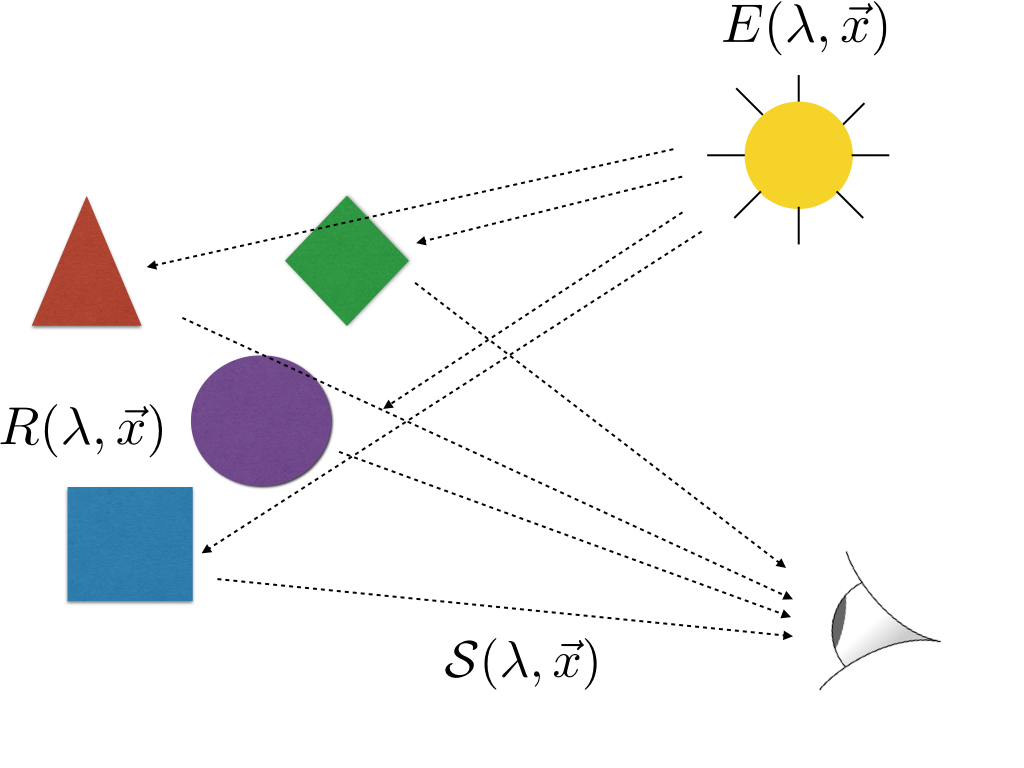
\includegraphics[width=\textwidth]{../FiguresDraft5/Figure1/Figure1_a.png}
        \label{fig:introSchematic}
    \end{subfigure}
    \begin{subfigure}{0.55 \textwidth}   
        \caption{}    
        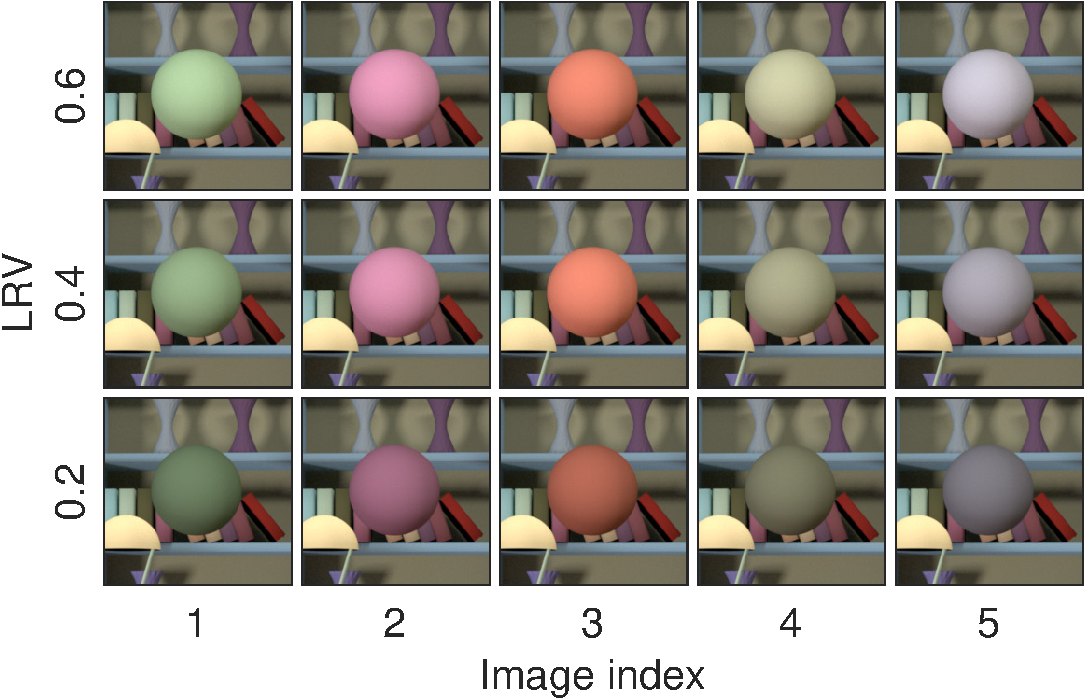
\includegraphics[width=\textwidth]{../FiguresDraft5/Figure1/Figure1_b.pdf}
        \label{fig:introExampleFigure}
    \end{subfigure}
    \label{introFigure}
    \caption{{\bf Color and luminance constancy:} (a)  The light reflected from an object to the eye depends both on the surface reflectance of the object and on the illumination of the object. 
The reflected light also depends on geometric factors, such as the object's shape, pose, and position. 
The human visual system accounts for variations in the reflected light due to object-extrinsic factors and produces a percept of object color that is relatively stable across such variations, an ability called color constancy. 
(b) Images of a sphere under a fixed illuminant.  
Down each column, the sphere's light reflectance value (LRV) varies, but the relative reflectance spectrum (i.e. its spectral shape) is held fixed.
Across each row, the relative reflectance spectrum varies, but the LRV is held fixed.
We cast the problem of computational luminance constancy to be that of estimating the LRV of a target object from the image, across variation in other scene factors. 
Specifically, we study variation in target object relative surface reflectance, variation in illumination spectrum, and variation in the surface reflectance of the other objects in the scene.}
 \end{figure}

Recently, supervised statistical learning methods have been applied to the computational problem of color constancy.
These methods use the joint statistics of labeled images and scene variables to learn mappings that extract stable surface color descriptors from image input \cite{barron2015convolutional}.
This general statistical learning approach has been useful for other perceptual problems in early and mid-level vision.
For example, a recently developed technique called accuracy maximization analysis (AMA) learns linear filters optimized for particular perceptual tasks \cite{geisler2009optimal,burge2017accuracy,jaini2017linking}. It has been used to develop ideal observers for defocus blur, binocular disparity, and retinal motion estimation with natural stimuli that provide excellent predictions of neural and human performance \cite{burge2011optimal, burge2012optimal, burge2014optimal, burge2015optimal}.
In this paper, we apply AMA to a special case of computational color constancy. 

Supervised learning requires large labeled data sets.  Such data sets are not readily available for the study of color constancy. Although there are datasets of calibrated color images, these datasets do not provide ground truth information about surface reflectance and illumination at each image location \cite{ChakrabartiHyperspectral,NascimentoFoster2016,ParragaHyperspectralData,TkacikUpennHypersepctralData,skauli2013collection,olmos2004biologically}. There are a few databases consisting of images of posed scenes where object surface reflectances are measured individually (\citeNP{funt1988color,ciurea2003large}), but these are not large enough to drive supervised learning.
 
In this paper, we use high-quality computer graphics to generate large datasets of naturalistic images where the surface reflectance corresponding to each image pixel is known. 
This approach allows us to investigate computational color constancy with naturalistic stimuli, while retaining the ability to control the properties of objects and illuminants. We use this approach to tackle the specific problem of luminance constancy, a constitutive component of the more general color constancy problem (Fig.~\ref{fig:introExampleFigure}). 

We define the computational problem of luminance constancy as that of estimating the light reflectance value (LRV) of a target object's surface reflectance function.
The LRV is a measure of the overall amount of light reflected by a surface \cite{astm1121477}.
Computation of an LRV from a surface reflectance function proceeds in two steps.
First, we computed the luminance of the light that would be reflected from the surface under a reference illuminant.
Second, we normalize the result by the luminance of the reference illuminant itself.
Here we use CIE daylight D65 as the reference illuminant and the CIE 1931 photopic luminosity function to compute luminance \cite{CIE86}.
Sometimes LRVs are expressed as a percentage.
Here we express LRVs as proportion, so that they take on values between 0 and 1.

\section*{Methods} \label{Methods}
% Figure 2
\begin{figure}
\centering
\begin{subfigure}[b]{0.22 \textwidth}
        \caption{Library }
        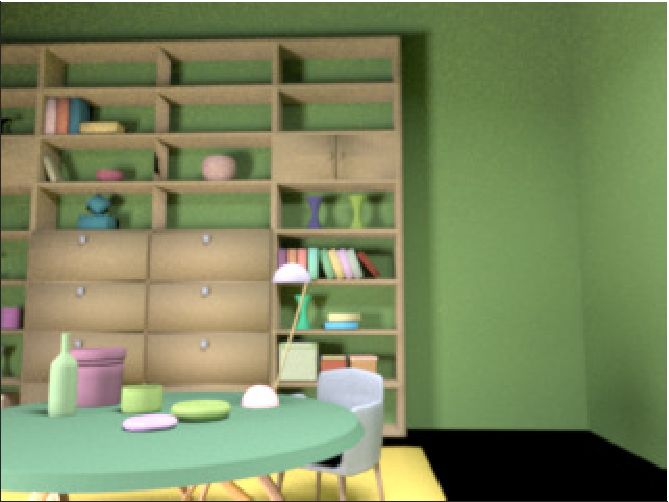
\includegraphics[width=\textwidth]{../FiguresDraft5/Figure2/Figure2_a.pdf}
        \label{fig:baseSceneLibrary}
    \end{subfigure}
    ~
    \begin{subfigure}[b]{0.22 \textwidth}
        \caption{Mill}    
        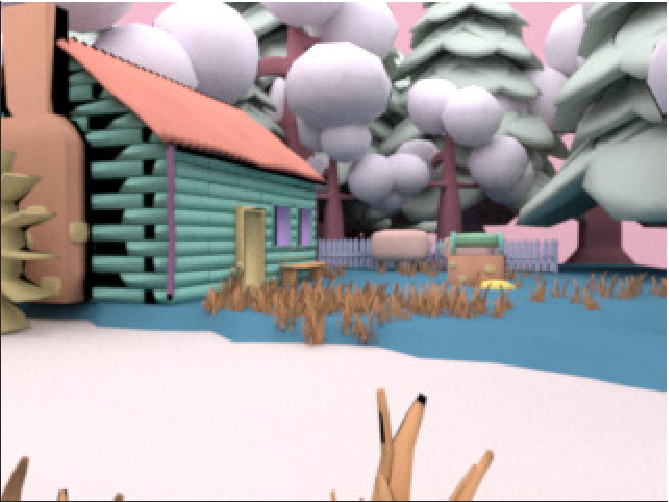
\includegraphics[width=\textwidth]{../FiguresDraft5/Figure2/Figure2_b.pdf}
        \label{fig:baseSceneMill}
    \end{subfigure}    
    ~
    \begin{subfigure}[b]{0.22 \textwidth}
        \caption{Table-Chairs}    
        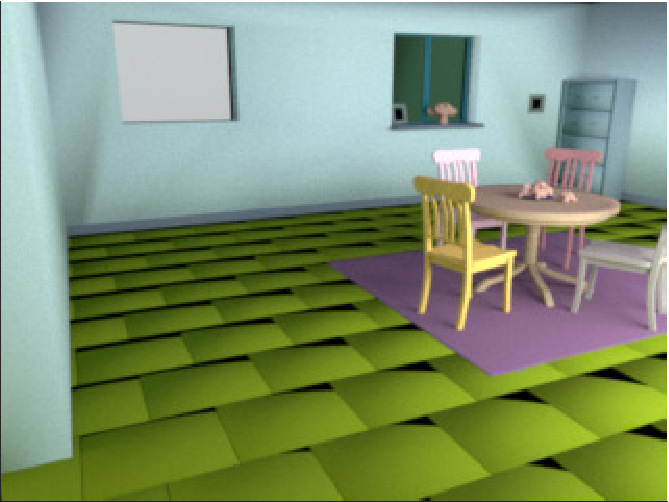
\includegraphics[width=\textwidth]{../FiguresDraft5/Figure2/Figure2_c.pdf}
        \label{fig:baseSceneTableChairs}
    \end{subfigure}
    \caption{{\bf Base scenes.} Each subplot shows a rendering of one base scene without additional inserted objects.  The reflectance spectra of the distinct surfaces and the spectral power distributions of the light sources in each scene have been assigned randomly from statistical models of naturally occurring spectra (see text). The images in this figure have been scaled and tone mapped individually for illustrative purposes.}
\label{fig:baseScenes}. \end{figure}

\subsection{Overview}
There are four key parts to our methods.  First, we generate a labeled set of training images.  Second, we use a model of the early visual system to compute the responses of the cone photoreceptor mosaic to the labeled images. Third, we apply AMA to the cone responses, as well as to a contrast normalized version of the cone responses, to learn task-optimal receptive fields (RFs). Fourth, we evaluate how well the responses of the RFs may be decoded to achieve luminance constancy.


\subsection{Labeled training data} \label{method:VirtualWorld}
\subsubsection{Virtual naturalistic scenes}
The light that reflects from objects to the eyes depends on many factors.
These include the surface reflectance, texture, material and geometry of the objects, 
the spectral power distribution function of the illuminants, and the position of the observer.
We have developed a rendering package 
(\href{https://github.com/BrainardLab/VirtualWorldColorConstancy}{https://github.com/BrainardLab/VirtualWorldColorConstancy}) 
that allows us to construct models of naturalistic scenes, with key scene factors under programmatic control.
The package builds on our RenderToolblox4 package (\href{http://rendertoolbox.org}{http://rendertoolbox.org}) \cite{heasly2014rendertoolbox3},
and harnesses the open-source computer graphics renderer Mitsuba (\href{https://www.mitsuba-renderer.org}{https://www.mitsuba-renderer.org}, 
\citeNP{jakob2015mitsuba}) to produce physically-accurate images from the scene models.
Because each image is rendered from a known scene model, each image pixel can be labeled with 
the surface reflectance of the corresponding scene object.
By incorporating statistical models of the variation of object surface reflectance and daylight illumination, 
the pipeline allows us to produce large labeled sets of images that capture key aspects of the task-relevant 
statistical structure of natural scenes.

% Figure 3
\begin{figure}
\centering
    \begin{subfigure}[b]{0.14 \textwidth}
        \caption{Big-ball}
        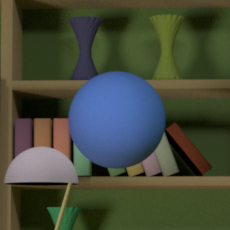
\includegraphics[width=\textwidth]{../FiguresDraft5/Figure3/Figure3_a.png}
        \label{fig:libraryWithBigBall}
    \end{subfigure}
     ~ 
    \begin{subfigure}[b]{0.14 \textwidth}
        \caption{Xylophone}
        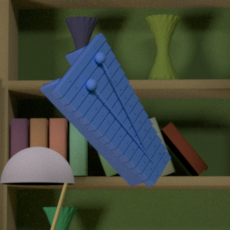
\includegraphics[width=\textwidth]{../FiguresDraft5/Figure3/Figure3_b.png}
        \label{fig:libraryWithXylophone}
    \end{subfigure}
     ~ 
    \begin{subfigure}[b]{0.14 \textwidth}
        \caption{Barrel}
        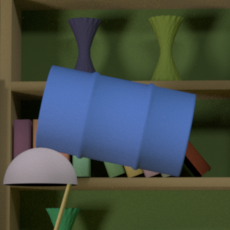
\includegraphics[width=\textwidth]{../FiguresDraft5/Figure3/Figure3_c.png}
        \label{fig:libraryWithBarrel}
         \end{subfigure}
    ~
	\begin{subfigure}[b]{0.14 \textwidth}
        \caption{Ring toy}
        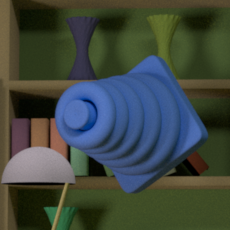
\includegraphics[width=\textwidth]{../FiguresDraft5/Figure3/Figure3_d.png}
        \label{fig:libraryWithRingToy}
    \end{subfigure}
        ~
    	\begin{subfigure}[b]{0.14 \textwidth}
        \caption{Bottle}
        
\includegraphics[width=\textwidth]{../FiguresDraft5/Figure3/Figure3_e.png}
        \label{fig:libraryWithChampagneBottle}
    \end{subfigure}
\caption{{\bf Library base scene with inserted objects.} The rendering package can be used to insert objects into base scenes. Each image (a-e) shows a different object inserted into a user specified location in the library base scene. The rendering viewpoint was set so that the object was at the center of the rendered image. The full rendered image has been cropped here so that the inserted object is easily visible.}\label{fig:libraryWithTarget}
\end{figure}

Our rendering package includes a collection of base scenes (Fig.~\ref{fig:baseScenes}).
Base scenes specify an arrangement of objects and light sources.
Base scenes may be enriched by the insertion of additional objects, chosen from an object library (Fig.~\ref{fig:libraryWithTarget}), and additional light sources.
Once the position, size and pose of the inserted objects and light sources have been set, 
a surface reflectance function can be assigned to each object in the scene, and a spectral power distribution function can be assigned to each light source (Fig.~\ref{fig:VWCCTransformations}). The resulting scene model can then be rendered from any specified viewpoint.

In the present work, we used our package to generate datasets of naturalistic scenes and corresponding images.
We used one fixed base scene and inserted a spherical target object of fixed shape and size into this scene.
We generated three distinct datasets, which we refer to as Conditions 1-3 and describe below.
Across these datasets the luminance constancy problem (i.e. estimating the target object LRV)
becomes progressively more difficult (Fig.~\ref{fig:studiedCases}).

The variation within our datasets captures the essence of the computational problem of lightness constancy
up to effects of scene geometry, an additional richness that we do not address in this paper.
In Condition 1, the relative reflectance spectrum of the target object was the only source of scene variation other than the target object LRV.
The reflectance spectra of the background objects, and the spectral power distributions of the light sources were kept fixed.
In Condition 2, the spectral power distribution of the light sources varied in addition to the relative reflectance spectrum of the target object,
Finally, in Condition 3 three distinct scene factors--target object relative reflectance spectrum, reflectance spectra of the background objects, and
spectral power distribution of the light sources--varied in addition to the target object LRV.
Conditions 1 and 2 had datasets consisting of 1000 scenes and images, 100 for each of 10 target object LRV values. 
Condition 3 had a dataset consisting of 3000 scenes and images, 300 each for the 10 target LRV values.
The LRV values were equally spaced between 0.2 and 0.6. For each LRV value, we generated a different target surface reflectance spectra for each of the 100 scenes. Thus, for each target object LRV value, the relative reflectance spectrum of the target object could differ.

% Figure 4
\begin{figure}
	\begin{subfigure}{0.18 \textwidth}
    \centering
        \caption{Target position}
        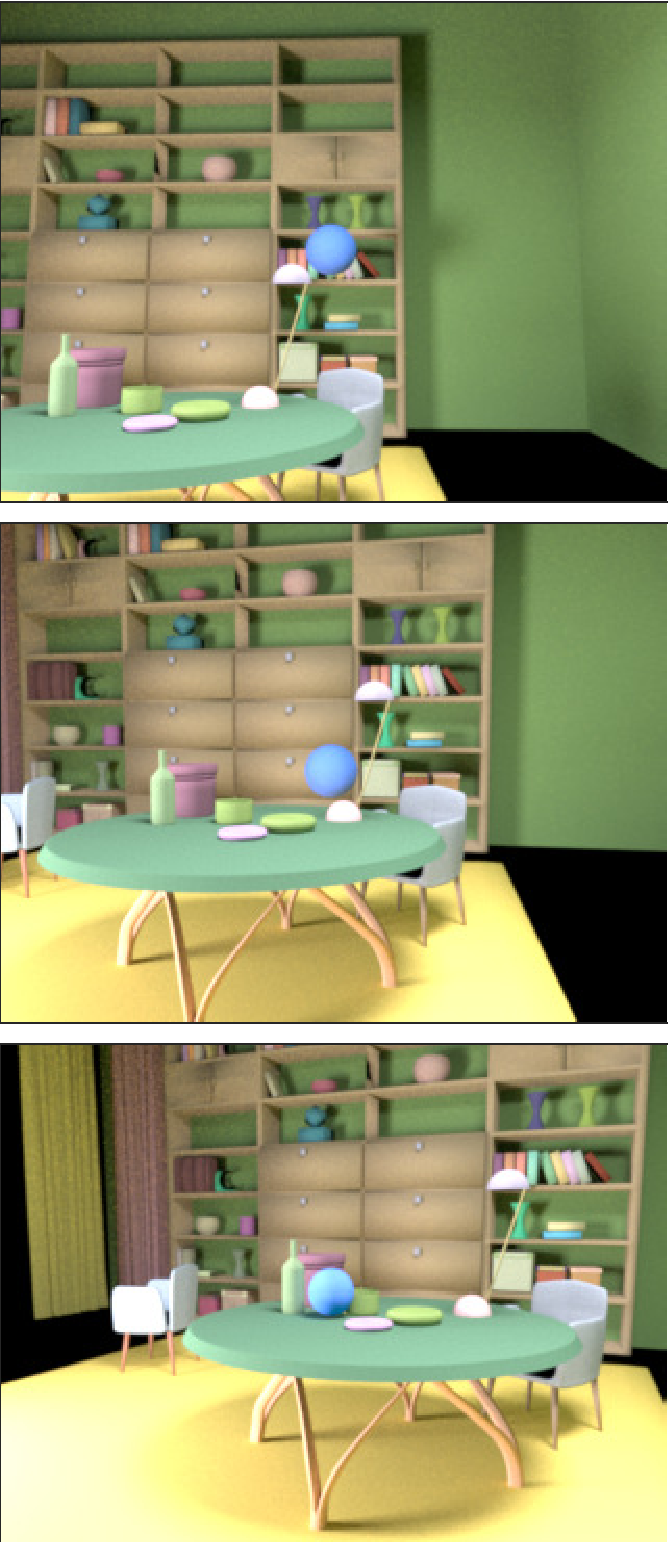
\includegraphics[width=\textwidth]{../FiguresDraft5/Figure4/Figure4_a.pdf}
        \label{fig:targetPositionVariation}
    \end{subfigure}
    ~
	\begin{subfigure}{0.18 \textwidth}
    \centering
        \caption{Target size/Orientation}
        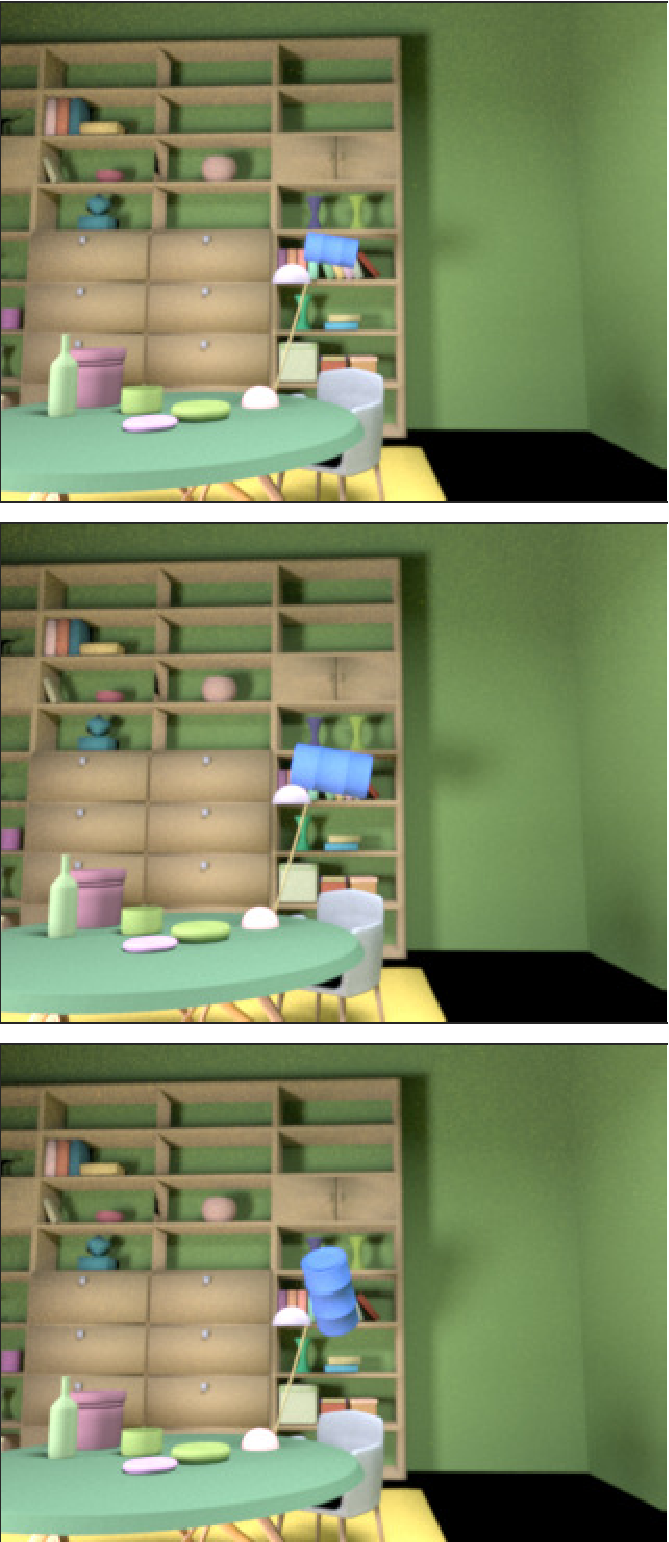
\includegraphics[width=\textwidth]{../FiguresDraft5/Figure4/Figure4_b.pdf}
        \label{fig:targetSizeOrientation}
    \end{subfigure}
~
\centering
	\begin{subfigure}{0.18 \textwidth}
    \centering
        \caption{Target spectra}
        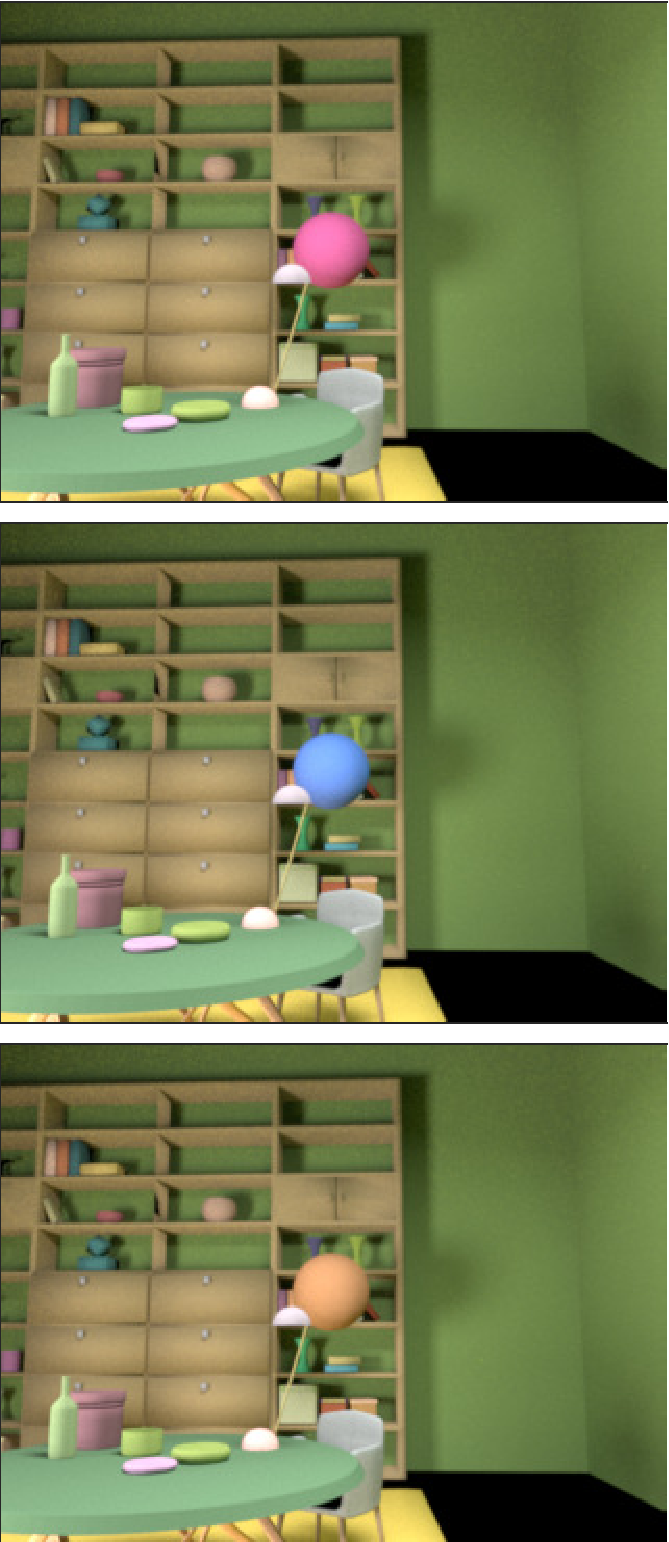
\includegraphics[width=\textwidth]{../FiguresDraft5/Figure4/Figure4_c.pdf}
        \label{fig:targetVariation}
    \end{subfigure}
    ~
    \begin{subfigure}{0.18 \textwidth}
    \centering
        \caption{Illumination spectra}
        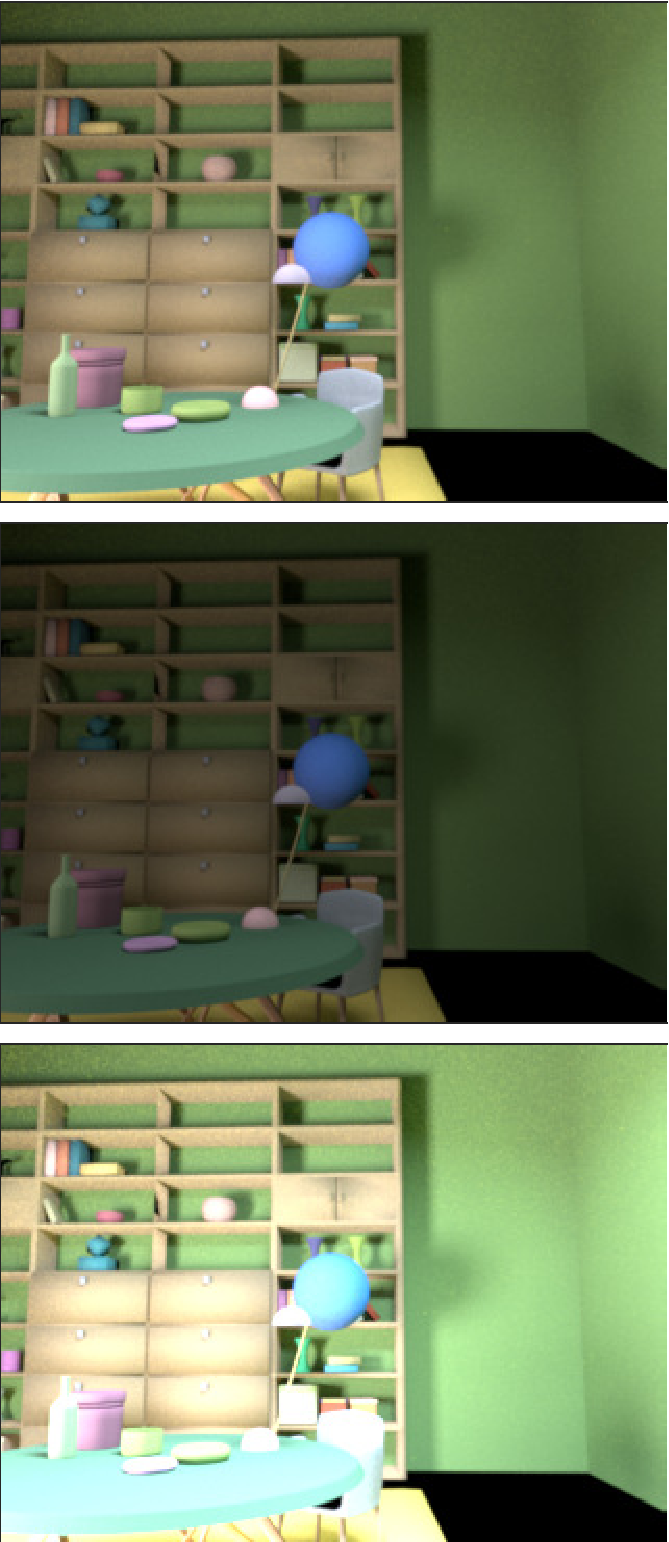
\includegraphics[width=\textwidth]{../FiguresDraft5/Figure4/Figure4_d.pdf}
        \label{fig:illuminationVariation}
    \end{subfigure}
          ~  
    \begin{subfigure}{0.18 \textwidth}
    \centering
        \caption{Background spectra}
        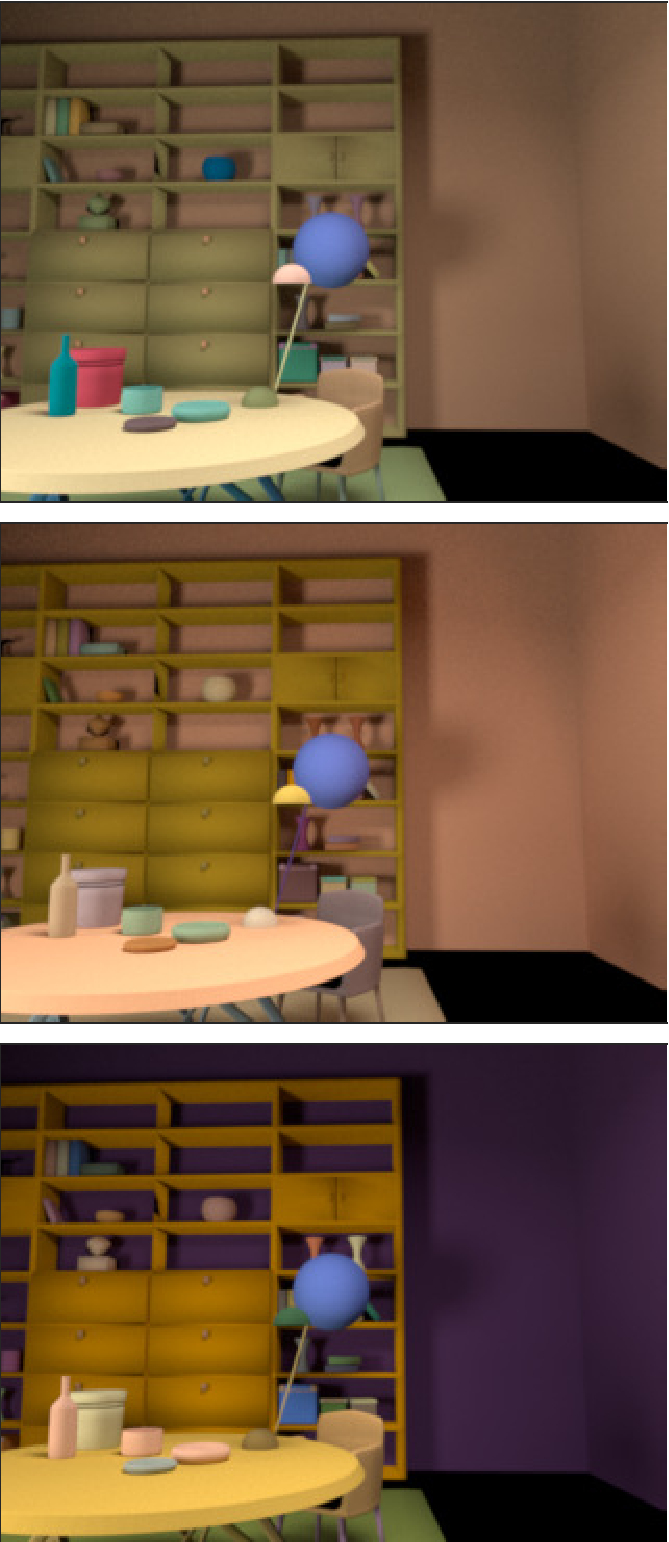
\includegraphics[width=\textwidth]{../FiguresDraft5/Figure4/Figure4_e.pdf}
        \label{fig:backGroundVariation}
    \end{subfigure}

    \caption{{\bf Scene transformations.} The properties of a visual scene can be broadly classified into two groups: geometrical (a-b) and spectral (c-e). Our rendering package provides control over the properties illustrated by the columns of the figure. (a) Variation in inserted object positions. (b) Variation in object pose. (c) Variation in the surface reflectance of the target object. (d) Variation in the spectral power distributions of the light sources. (e) Variation in surface reflectance of the background objects. All panels in this figure are rendered with a common scale factor and tone mapping.
\label{fig:VWCCTransformations}}
\end{figure}

For the primary results, we used the ``{\it Library}'' base scene and a spherical target object.
The library base scene contains 2 area lights. 
We inserted one additional spherical light source into the scene.
The position and size of the inserted object, inserted light source and viewpoint were held fixed across all 
scenes in the database. The geometry is shown in Figure~\ref{fig:3DScene}.
Surface and illuminant spectra were drawn according to statistical models of naturally occurring spectra, as described below.
Multispectral images ($320 \times 240$ pixels) were rendered at 31 evenly-spaced wavelengths between $400$nm and $700$nm.

% Figure 5: Conditions Studied
\begin{figure}
\centering
	\begin{subfigure}{0.33 \textwidth}
		\caption{Condition 1}
%		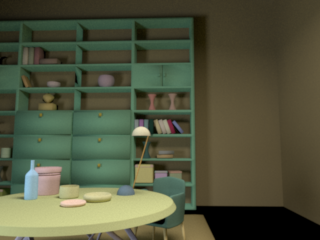
\includegraphics[width=\textwidth]{../FiguresDraft5/Figure2/Figure2_a.png}
		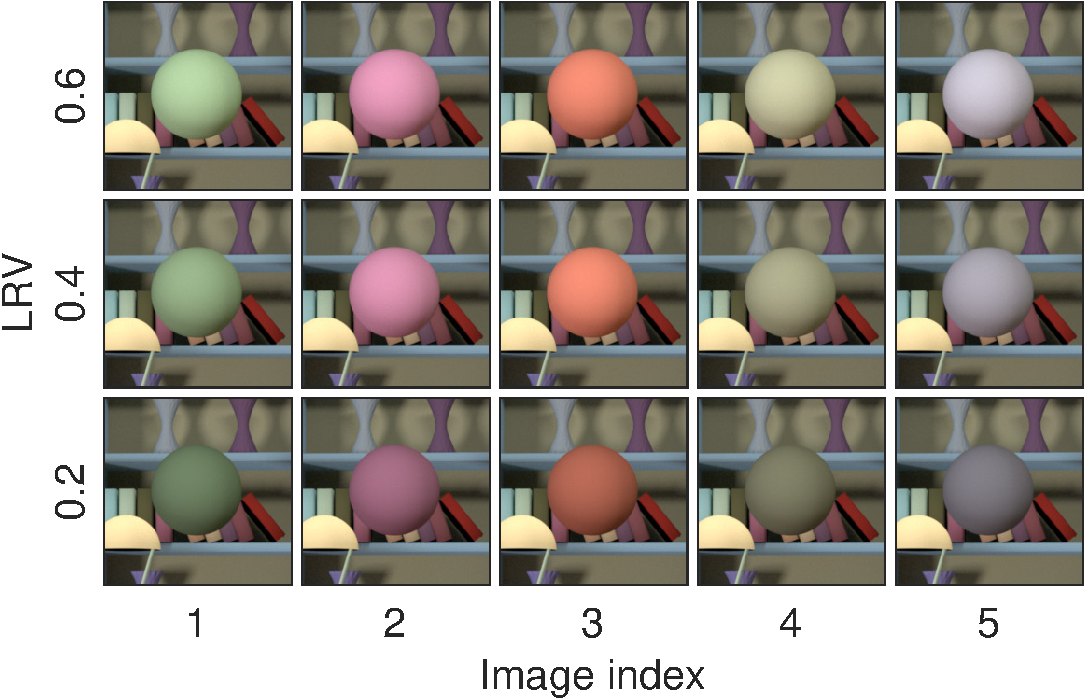
\includegraphics[width=\textwidth]{../FiguresDraft5/Figure1/Figure1_b.pdf}
 		\label{fig:backgroundVarying}
	\end{subfigure}
	\begin{subfigure}{0.33 \textwidth}
        \caption{Condition 2}	
        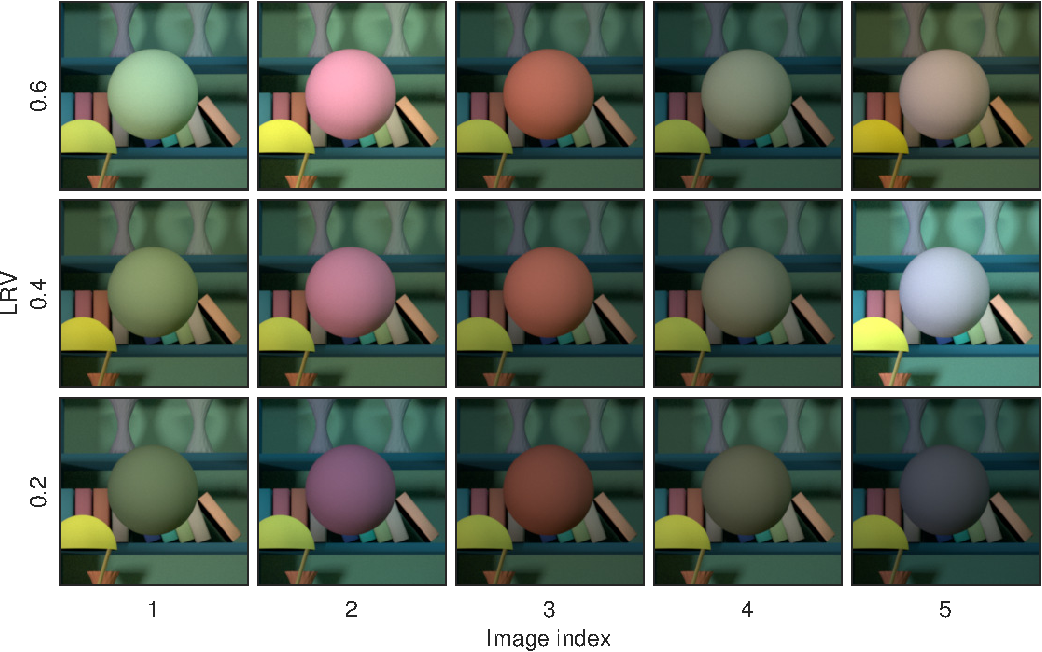
\includegraphics[width=\textwidth]{../FiguresDraft5/Figure5/Figure5_b.pdf}
        \label{fig:targetIlluminantVarying}
    \end{subfigure}
	\begin{subfigure}{0.33 \textwidth}
	\caption{Condition 3}	
        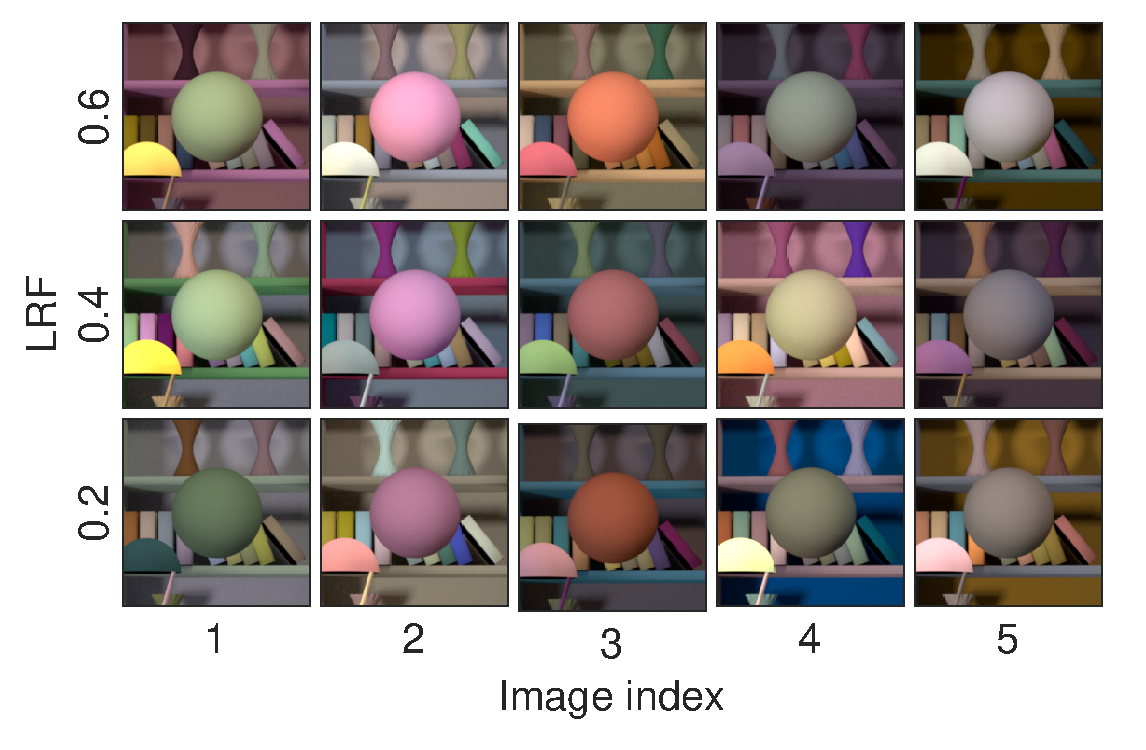
\includegraphics[width=\textwidth]{../FiguresDraft5/Figure5/Figure5_c.pdf}        
        \label{fig:allSpectraVarying}
    \end{subfigure}    
    \caption{{\bf Conditions 1-3:} sRGB renderings of illustrative images for the three types of spectral variations studied in this paper. (a) Condition 1: variable target object relative reflectance spectrum, fixed light source spectra, fixed background object spectra (same as Fig.~\ref{fig:introExampleFigure}). 
(b) Condition 2: variable target object relative reflectance spectrum, variable light source spectra, fixed background object spectra. (c) Condition 3: variable target object relative reflectance spectrum, variable light source spectra, variable background object spectra. The spheres in each row of each panel have the same LRV, while the spheres in each column of each panel have the same relative surface reflectance.  Across panels a-c, spheres in corresponding locations have the same surface reflectance. In all three panels, the overall light source spectra scale factors (see \nameref{Methods}) were drawn from a uniform distribution on the range [0.5, 1.5]. This is smaller than the variation we studied, but allows us to show the variation within the dynamic range available for display in publication. The sRGB values for all three subplots were tone mapped and normalized using a common scale factor prior to gamma correction.} 
\label{fig:studiedCases}
\end{figure}

\subsubsection{Illumination spectra}
To generate illumination spectra, we first developed a statistical model of the Granada daylight measurements (\citeNP{hernandez2001color}; \href{http://colorimaginglab.ugr.es/pages/Data}{http://colorimaginglab.ugr.es/pages/Data}) and then sampled randomly from the model (see appendix).
To match the wavelength spacing we use in rendering, we resampled the wavelength spacing of the Granada spectra to
31 evenly-spaced wavelengths between 400 nm and 700 nm.

% Figure 6
\begin{figure}
\centering
    \begin{subfigure}[b]{0.24 \textwidth}
    \centering
	\caption{Granada dataset}
        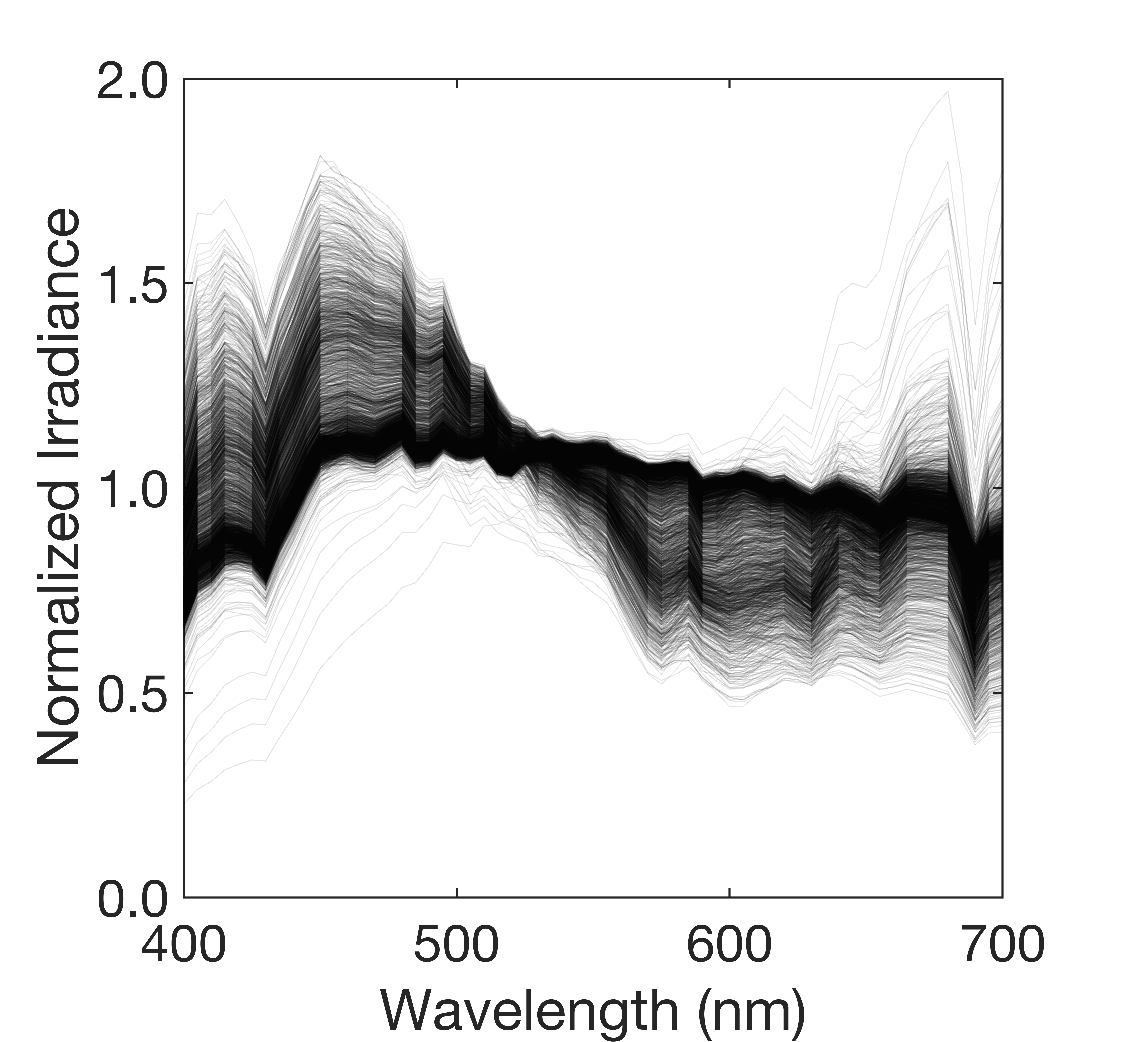
\includegraphics[width=\textwidth]{../FiguresDraft5/Figure6/Figure6_a.pdf}
        \label{fig:granadaData}
    \end{subfigure}
	\begin{subfigure}[b]{0.24 \textwidth}
    \centering
        \caption{Statistical model}
        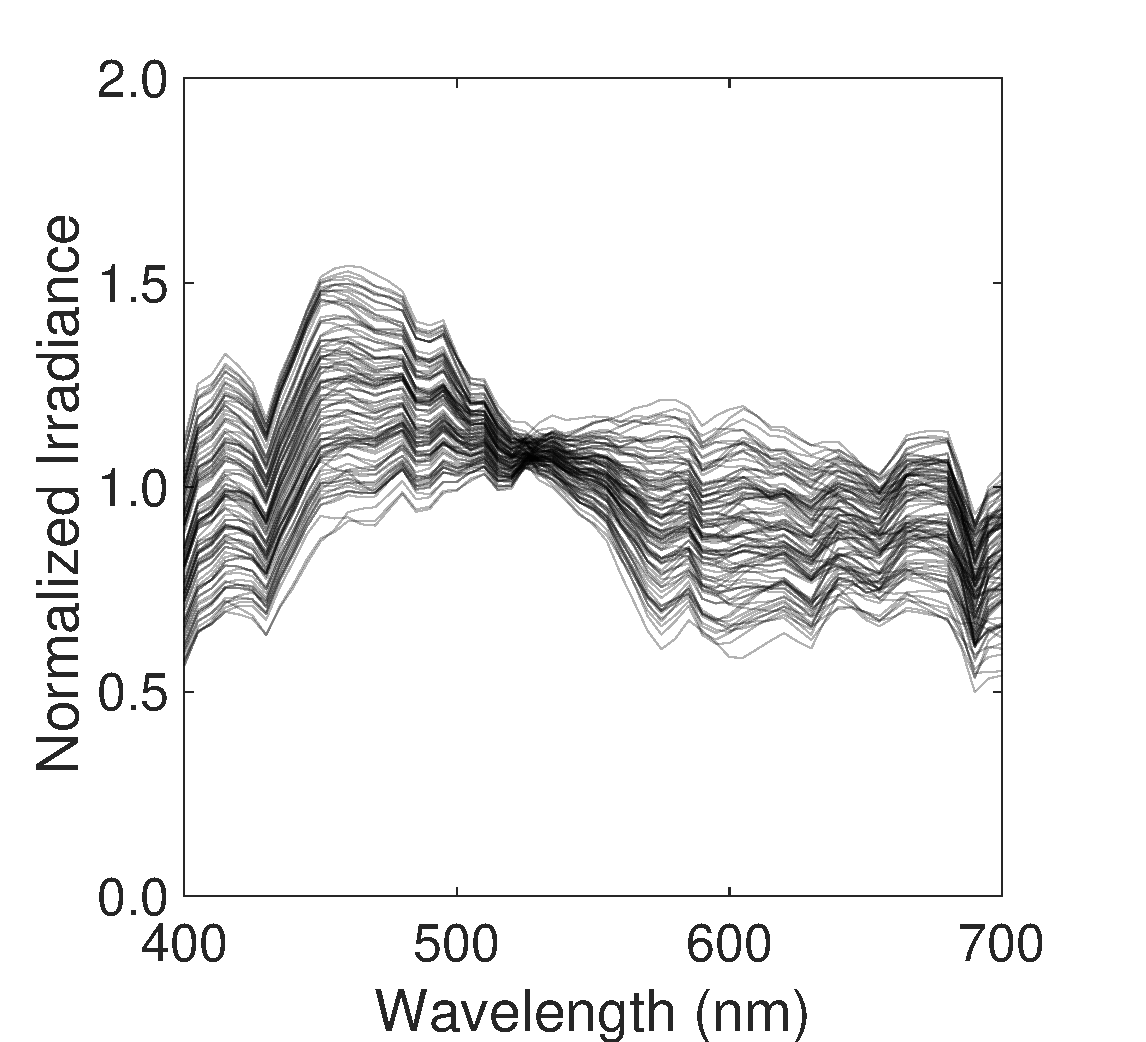
\includegraphics[width=\textwidth]{../FiguresDraft5/Figure6/Figure6_b.pdf}
        \label{fig:illuminantSamples}
    \end{subfigure}
      	\begin{subfigure}[b]{0.24 \textwidth}
    \centering
        \caption{CIE xy chromaticity}
        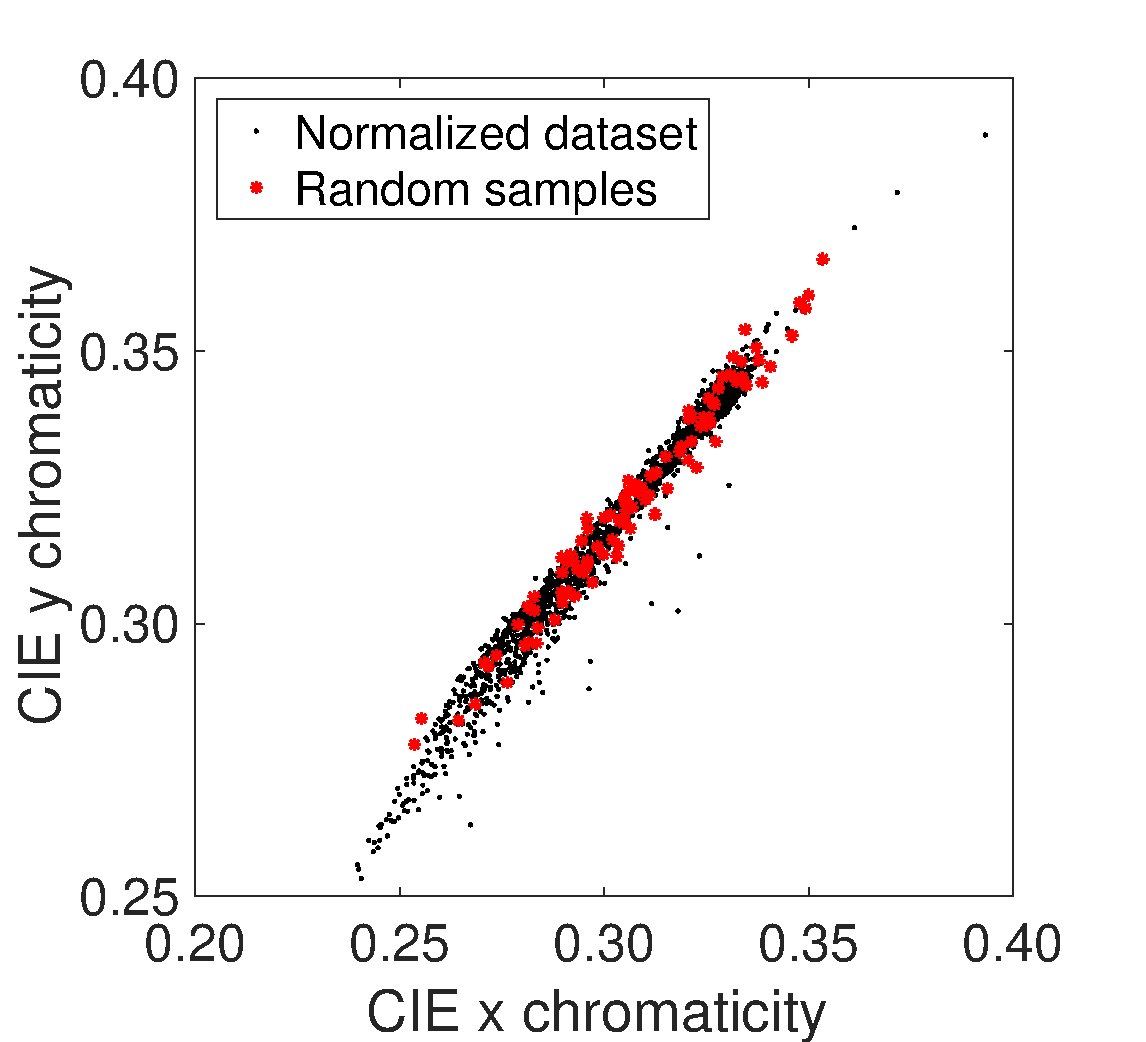
\includegraphics[width=\textwidth]{../FiguresDraft5/Figure6/Figure6_c.pdf}
        \label{fig:xyDiagram}
        \end{subfigure}
      	\begin{subfigure}[b]{0.24 \textwidth}
    \centering
        \caption{Color swatches}
        
\includegraphics[width=\textwidth]{../FiguresDraft5/Figure6/Figure6_d.pdf}
        \label{fig:sRGBIlluminant}
    \end{subfigure}
    \caption{{\bf Statistical model of illumination spectra:} (a) Normalized Granada dataset. Each spectrum is normalized by its mean power. (b) Sample spectra generated using the statistical model derived from normalized Granada dataset. (c) CIE xy chromaticities of the Granda dataset (black) and the samples shown in b (red). (d) sRGB renditions of the samples shown in b.}
\label{fig:illuminant}
\end{figure}

Our statistical model approximates the normalized Granada spectra using the first 6 principle components.
The variation in the weights on these components is modeled with a 6-dimensional Gaussian.
The mean and covariance matrix of the Gaussian match the sample mean and covariance of the weights \cite{BrainardFreeman}. 
To generate a random relative illuminant spectrum, we sample weights randomly from this Gaussian and then perform a weighted sum of the components to generate the corresponding spectrum.
Figure~\ref{fig:illuminantSamples} illustrates the relative spectra of draws obtained using this procedure.
Details of the statistical model for illumination are provided in the appendix.
Chromaticities and rendered color renditions of these draws are shown in Figures~\ref{fig:xyDiagram} and ~\ref{fig:sRGBIlluminant}.

Because our multivariate Gaussian model is based on normalized spectra, it does not embody the large variation in overall intensity of natural daylights.
To obtain illuminant spectra with intensity variation similar to the Granada dataset, we scaled each randomly generated spectrum with a random number sampled from a log-uniform distribution in the range [0.15, 150].
This procedure restores the three-order of magnitude intensity variation present in the original dataset.
We chose the particular scale factor range so that the mean number of cone isomerizations from the target object ranged from approximately 100 to 100,000 for the 100 msec cone integration time we used (see below).
This range corresponds approximately to that for natural viewing.

\subsubsection{Surface reflectance spectra}
% Figure 7 Surface Reflectance Data and Model
\begin{figure}
\centering
	\begin{subfigure}{0.24 \textwidth}
    \centering
            \caption{Munsell and Vrhel dataset}
        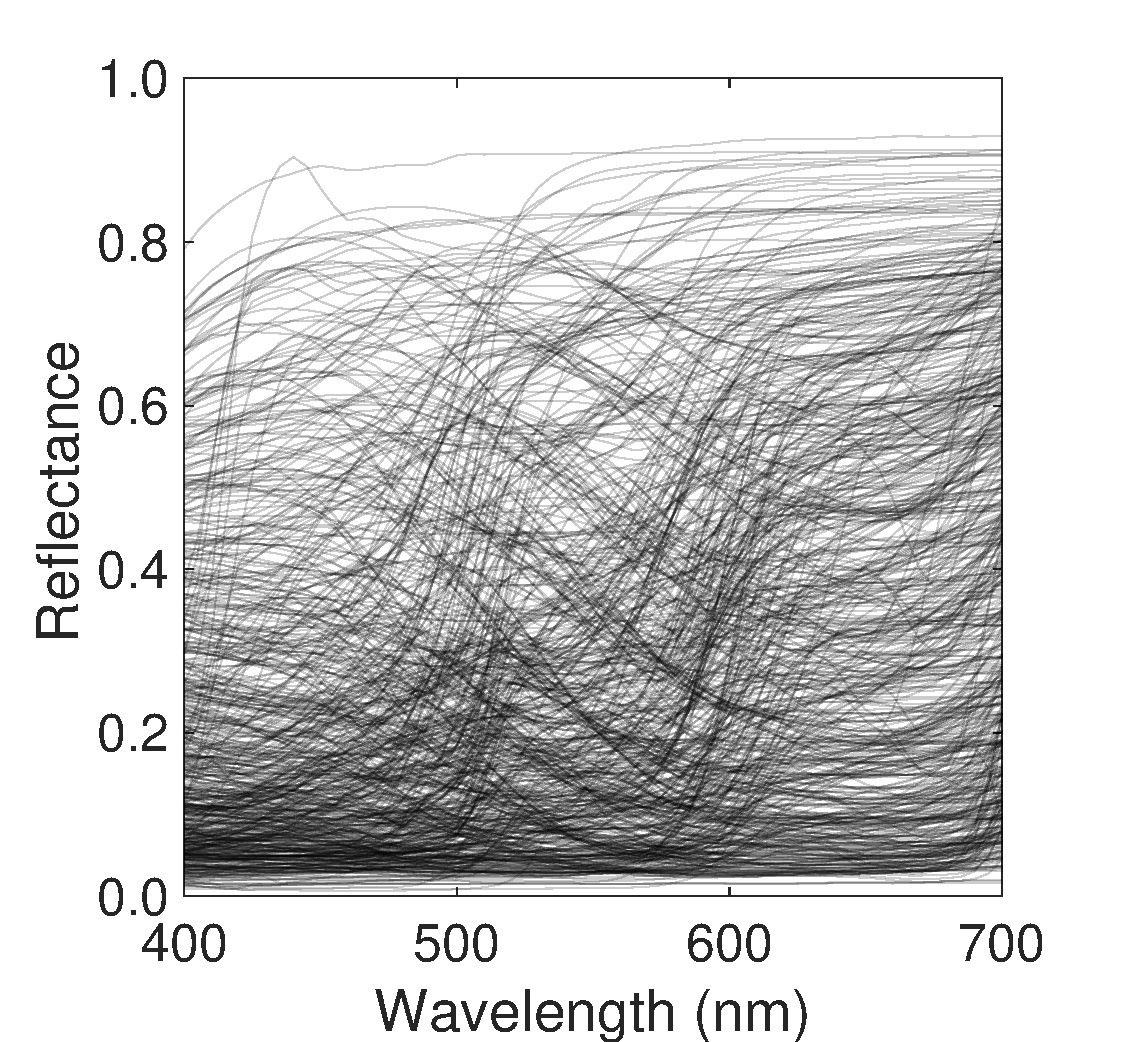
\includegraphics[width=\textwidth]{../FiguresDraft5/Figure7/Figure7_a.pdf}
        \label{fig:reflectanceSpectra}
    \end{subfigure}
    \begin{subfigure}{0.24 \textwidth}
    \centering
        \caption{Statistical model}
        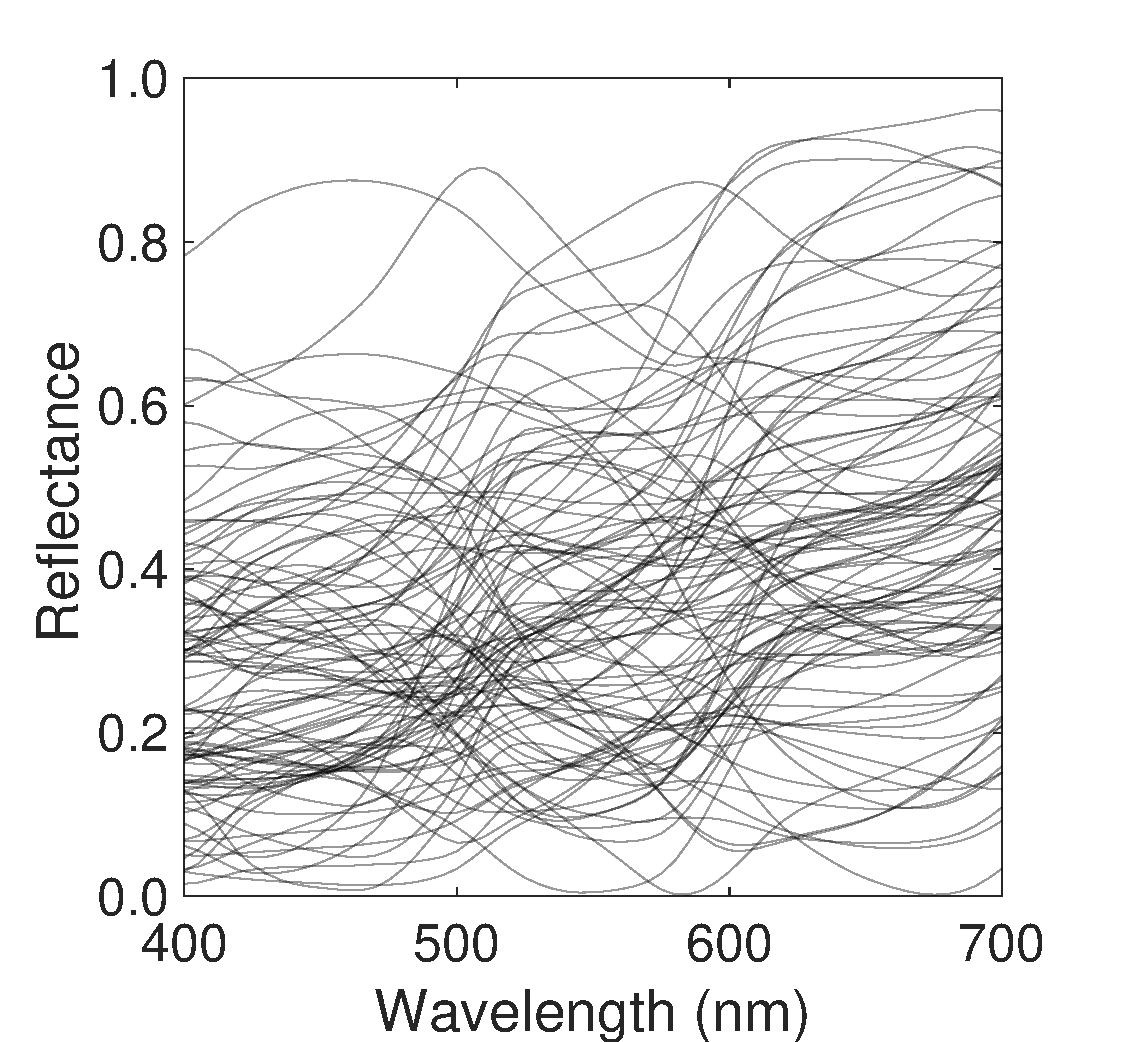
\includegraphics[width=\textwidth]{../FiguresDraft5/Figure7/Figure7_b.pdf}
        \label{fig:reflectanceSamples}
    \end{subfigure}
    \begin{subfigure}{0.24 \textwidth}
    \centering
    \caption{CIE xy chromaticity}
        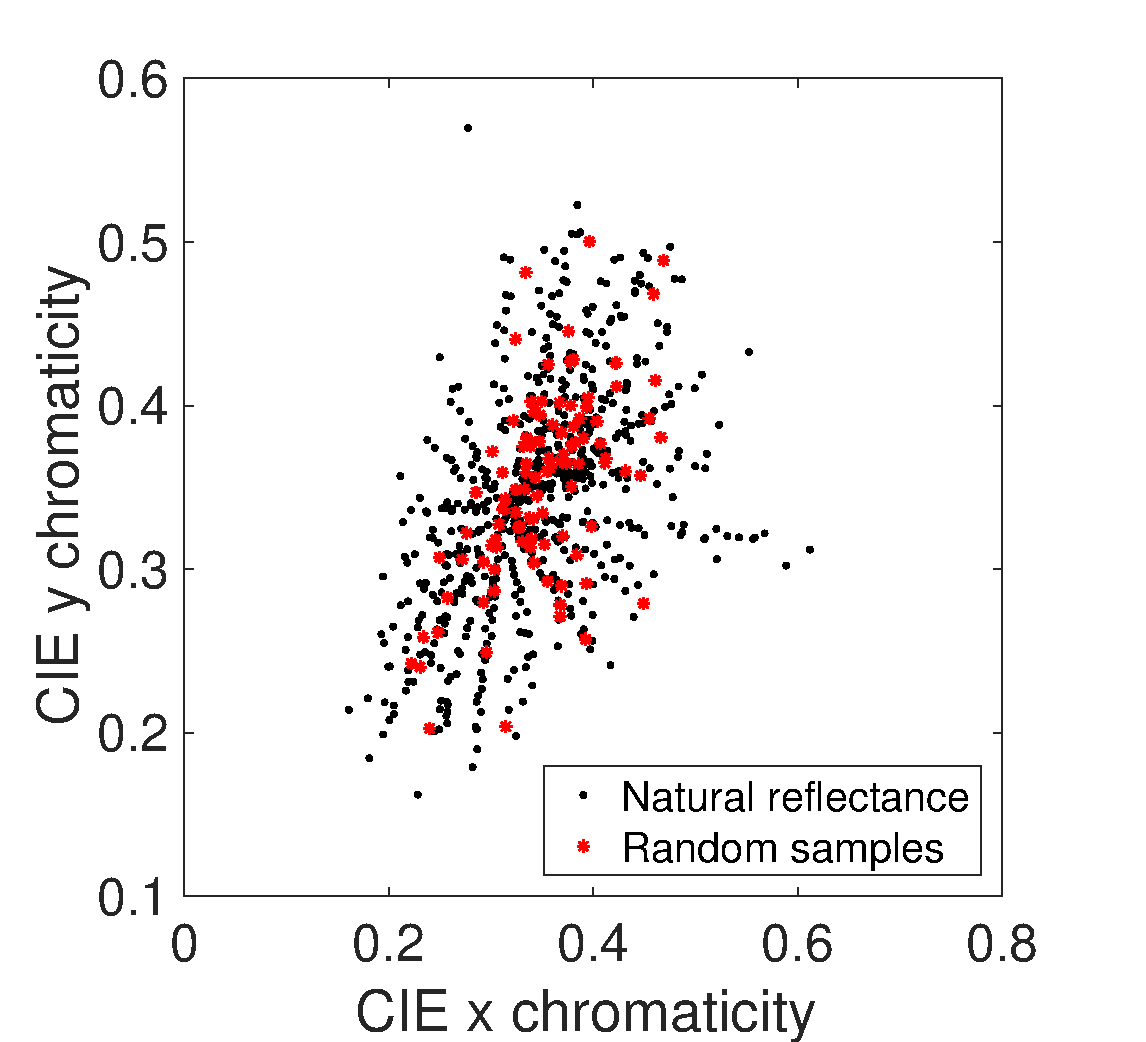
\includegraphics[width=\textwidth]{../FiguresDraft5/Figure7/Figure7_c.pdf}
        \label{fig:xyChroReflectance}
    \end{subfigure}    
    \centering
	\begin{subfigure}{0.24 \textwidth}
    \centering
        \caption{Color swatches}
        
\includegraphics[width=\textwidth]{../FiguresDraft5/Figure7/Figure7_d.pdf}
        \label{fig:backgroundSwatches}
    \end{subfigure}
    \caption{{\bf Statistical model of surface reflectance:} (a) Surface reflectance spectra from the Munsell and Vrhel datasets. (b) Sample spectra generated using the surface reflectance statistical model. (c) CIE xy chromaticity diagram of the Munsell and Vrhel reflectances and samples shown in b (red). (d) sRGB renditions of the samples shown in b, rendered under the CIE D65 daylight.}
\label{fig:surfaceReflectanceGeneration}
\end{figure}

%Figure 8 Target Surface Reflectance Samples
\begin{figure}
\centering
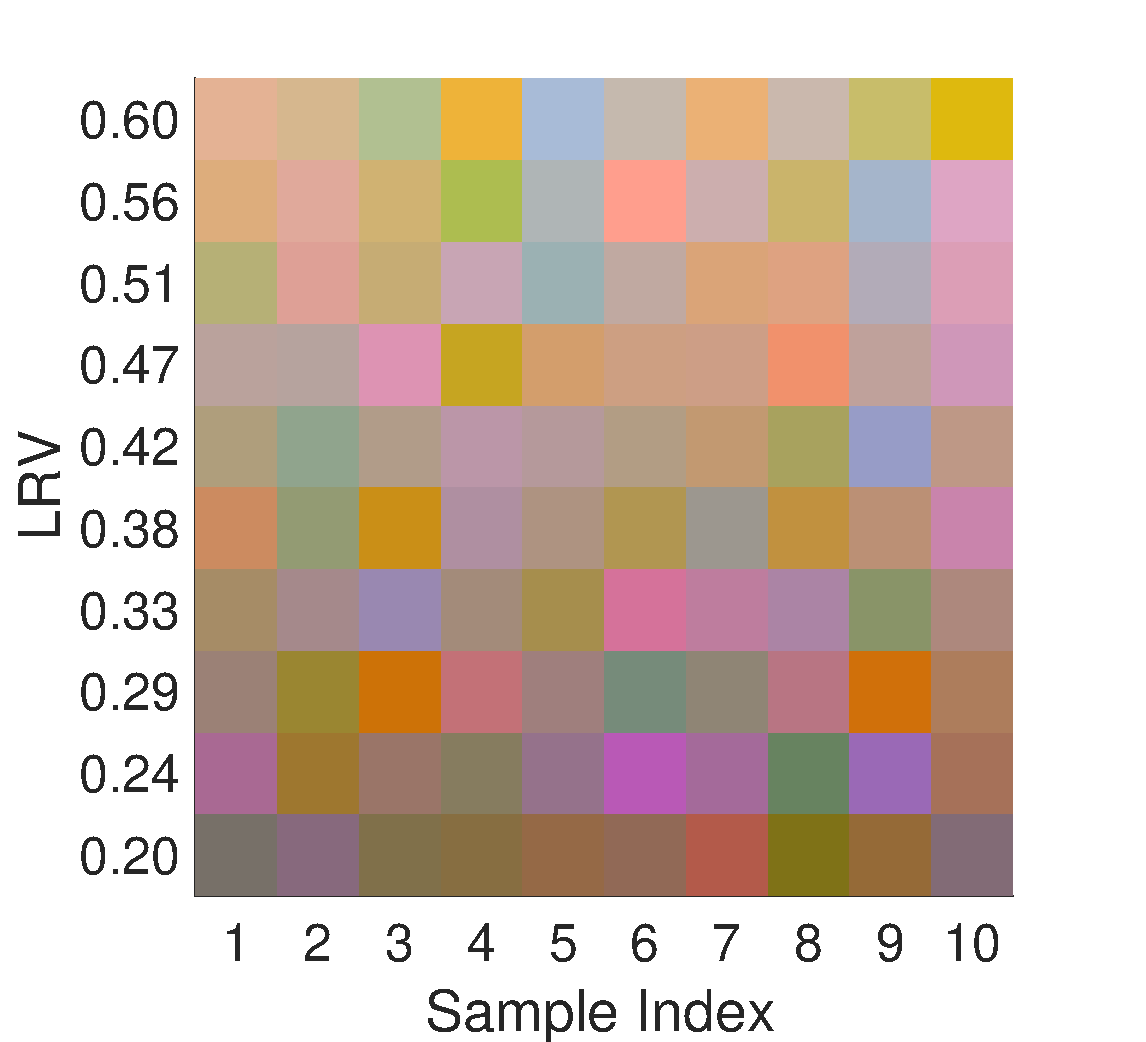
\includegraphics[width=0.3\textwidth]{../FiguresDraft5/Figure8/Figure8.pdf}
\caption{{\bf Target object surface reflectance spectra:} sRGB renditions of the target object surface reflectance rendered under CIE D65 daylight spectrum. The figure shows 10 random samples at 10 equally spaced LRV levels in the range [0.2, 0.6]. Each row contains 10 random samples of reflectance spectra generated at the LRV shown on the left.}
\label{fig:targetSwatches}
\end{figure}

To generate random reflectance spectra, we used the same principles we used to model illuminant spectral power distributions.
We combined the Munsell \cite{kelly1943tristimulus} and Vrhel \cite{vrhel1994measurement} surface reflectance 
measurements to create a database containing 632 reflectance spectra (462 from the Munsell data and 170 from the Vrhel data) (Figure~\ref{fig:reflectanceSpectra}).
We resampled the spectra to 31 evenly-spaced wavelengths between 400 nm and 700 nm (Figure~\ref{fig:reflectanceSpectra}).
Details of the statistical model for surface reflectance spectra are provided in the appendix. 
Figures~\ref{fig:reflectanceSamples},~\ref{fig:xyChroReflectance}, and~\ref{fig:backgroundSwatches} illustrate reflectance draws obtained using the model. 

For generating the target object reflectance at a particular luminance, the generated reflectance spectrum was 
scaled such that the LRV had the desired value (see appendix).
Figure \ref{fig:targetSwatches} shows color renderings of target reflectance spectra under CIE illuminant D65, for the evenly spaced LRV values we studied.

% Figure 8: Methods
\begin{figure}
\centering
\begin{subfigure}[b]{0.25 \textwidth}
		\centering
        \caption{sRGB rendering of a 3D scene}
        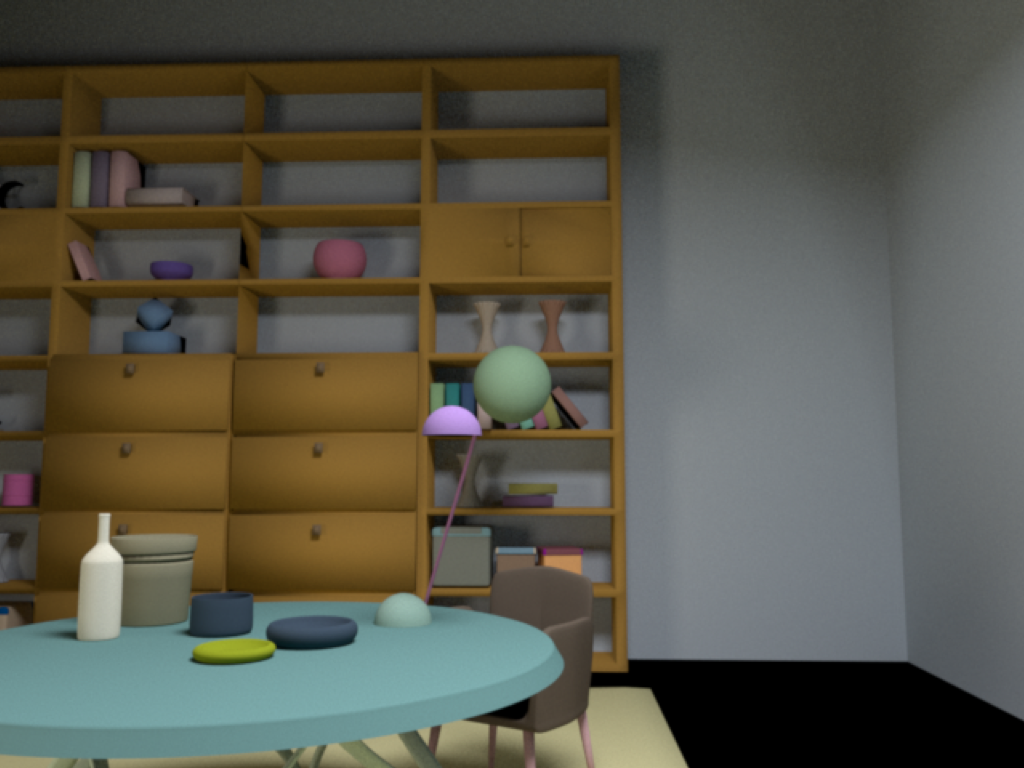
\includegraphics[width=\textwidth]{../FiguresDraft5/Figure9/Figure9_a.png}
        \label{fig:3DScene}
    \end{subfigure}
    ~ 
    \begin{subfigure}[b]{0.19 \textwidth}   
    \hspace{0.1 \textwidth}
        \caption{Cropped image}
        \vspace{1.5mm}
        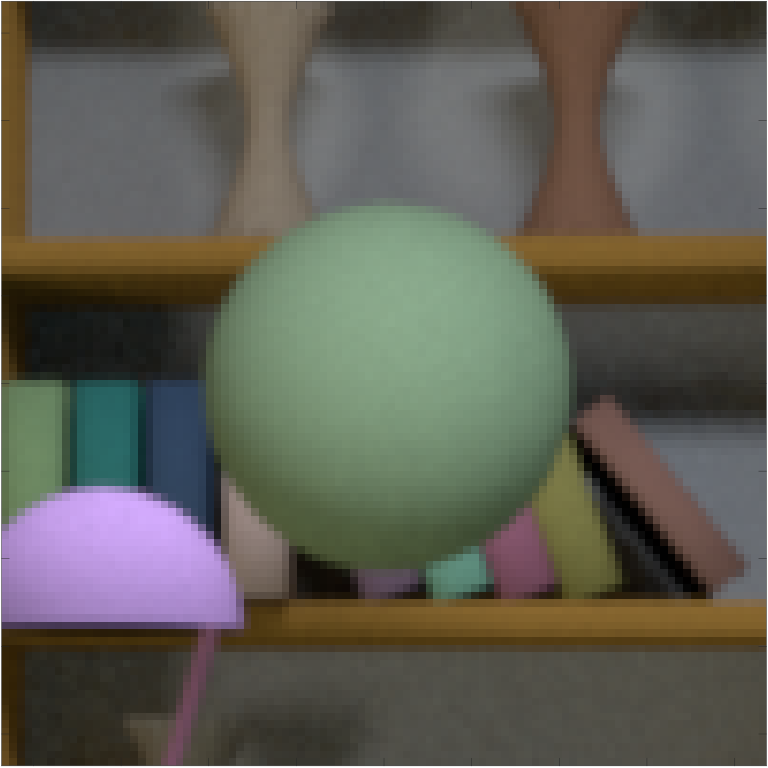
\includegraphics[width=\textwidth]{../FiguresDraft5/Figure9/Figure9_b.png}
        \label{fig:croppedImage}
    \end{subfigure}
    ~ 
    \begin{subfigure}[b]{0.19 \textwidth}
    \hspace{0.1 \textwidth}
        \caption{Retinal image}
        \vspace{1.5mm}
        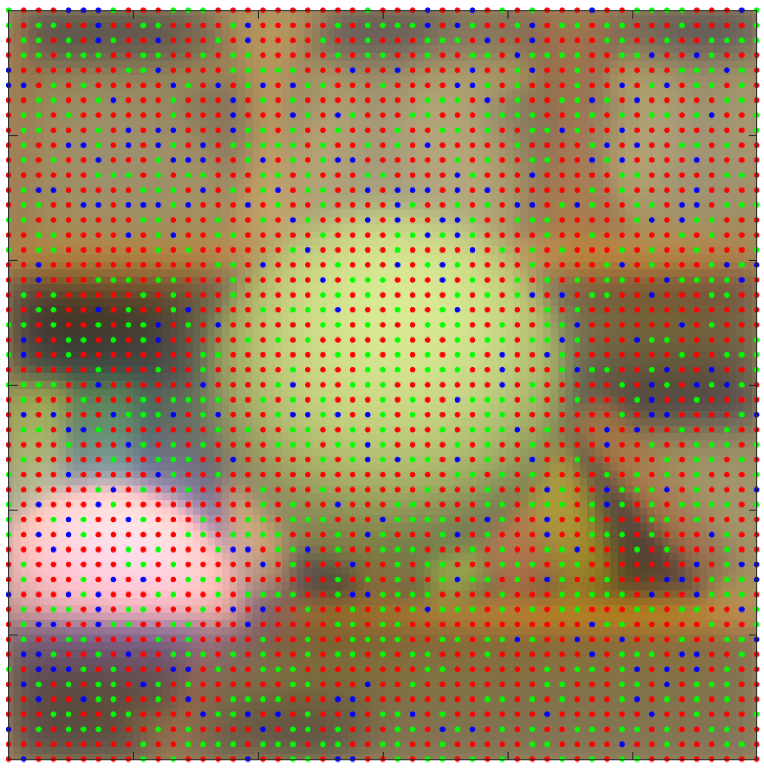
\includegraphics[width=\textwidth]{../FiguresDraft5/Figure9/Figure9_c.png}
        \label{fig:croppedImageWithMosaic}
    \end{subfigure}
    ~
    \begin{subfigure}[b]{0.2 \textwidth}
        \caption{Normalized cone contrast}
        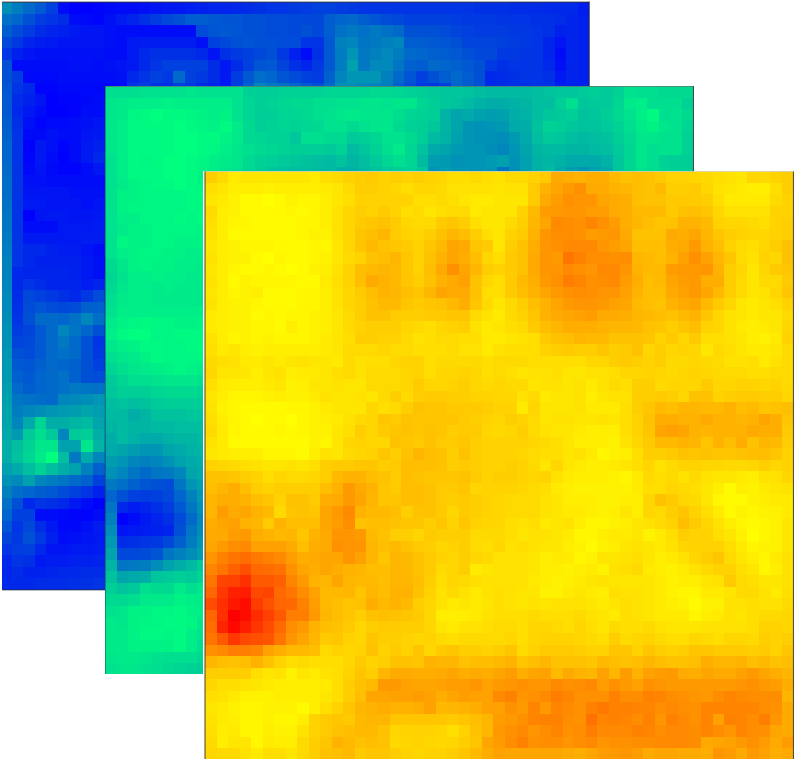
\includegraphics[width=\textwidth]{../FiguresDraft5/Figure9/Figure9_d.png}
        \label{fig:coneContrast}
    \end{subfigure}
    \label{fig:sceneWithCroppedImage}
    \caption{{\bf Pipeline for generating labeled datasets:}  The labeled images used in this paper are generated as follows: (a) A 3D virtual scene, containing a target object is created. The rendering viewpoint is selected so that the target object is in the center of the image. Spectra are assigned to the target object, illuminants, and other objects in the scene using the statistical models described in the text. A multispectral image of the scene is then rendered. (b) The central portion of the rendered image is cropped around the target object. (c) The retinal image corresponding to the rendered image is computed, which is then used to compute the number of photopigment isomerizations in the cone photoreceptors. The figure shows a rendering of the retinal image after optical blurring, with the location and identity of the cones indicated by an overlay (L cones: red, M cones: green, S cones: blue).  (d) The cone excitations are linearly interpolated to estimate the responses of all the three types of cone at each location (demosaicing). Finally, the demosaiced images are contrast normalized.}
\end{figure}

\subsection{Model of early visual system} \label{method:Isetbio}
The light entering the eye is blurred by the optics of the eye.
The resulting retinal image is sampled by a mosaic of cone photoreceptors.
The excitations of these photoreceptors provide the information about the scene that is available to the neural visual system for further processing.
Because we are interested in how well luminance constancy may be achieved by the human visual system, we simulated the cone excitations
to our scenes using a model of the early visual system.

We focussed our analysis on image regions local to the target by cropping the rendered images to $1 \times 1$ degrees of visual angle around the target object ($51 \times 51$ pixels; Figure~\ref{fig:croppedImage}). In foveal primary visual cortex, receptive fields have a spatial extent of approximately 1 degree of visual angle \cite{gattass1981visual, gattass1988visuotopic}. 
The local analysis is thus motivated by the fact that neural receptive fields early in the visual pathways (e.g., retina, primary visual cortex) pool information locally.

We modeled a visual system limited by diffraction caused by a 3mm diameter pupil, optical blurring (including axial chromatic aberration) in the formation of the retinal image \cite{marimont1994matching}, and spatial sampling by an interleaved mosaic of long (L), middle (M)  and short (S) wavelength-sensitive cones (\citeNP{brainard2015color}; Fig.~\ref{fig:croppedImageWithMosaic}). 
The cone mosaic contained L:M:S cones in the ratio 0.6:0.3:0.1 and with spectral sensitivities derived from the CIE physiological standard \cite{CIE86}.
Cone excitations were taken as the number of photopigment isomerizations, assuming an integration time of 100 msec. The Poisson nature of the photopigment isomerization was also included \cite{hecht1942energy}. 
This modeling was implemented using the software infrastructure provided by ISETBio (\href{https://isetbio.org}{https://isetbio.org}).

%% Details on ISETBIO computations from Nicolas (TEXT IN CAPS IS FROM VIJAY)
%% Scene: 
%%- the default mean luminance was set to 200, but there is a key-value param that could have overridden this value. 
%%  I do not know if this were the case.
%%
%% % MEAN LUMINANCE = 0, NO SCALING
%
%%- The default FOV was 1 deg, but there is a key-value param that could have overridden this value.
%%  I do not know if this were the case.
%%
%% % HORIZONTAL FOV = 1
%%
%%- Distance default is 1 meter, but there is  a key-value param that could have overridden this value.
%%  I do not know if this were the case.
%%
%%% DISTANCE 1M
%%
%%Optics: 
%%- 3 mm pupil, 17 mm focal length, with a spectro-spatial OTF described in  
%%  (Marimont & Wandell (1994) J. Opt. Soc. Amer. A,  v. 11, p. 3113-3122), 
%%   which includes axial chromatic aberration. However, there is key-value param o skip the OTF. 
%%   Not sure if this was used.  It it was used, the optics was set to diffraction limited.
%%
%% % SKIP OTF OFF:  'skipOTF', false ...  
%%
%%Lens: 
%%- not sure if the optical density is from Wyszecki&Stiles or from Stockman-Sharpe. 
%%  The isetbio file commend only says it is from PTB. David do you know, or should I check
%%  the data?
%%
%%Cone Mosaic: 
%%- rectangular cone mosaic with 0.6:0.3:0.1 LMS densities
%%- FOV was a key-value param, so I do not know what was used.
%%- Also the mosaic was subsampled  according to a cone-stride param, with a default of 15 cones
%%but there is a key-value param that could have overridden this value. I do not know what that parameter value was.
%%
%% CONE STRIDE = 3 'coneStride', 3, ... 
%%
%%
%%- There is a key-value pair to also low-pass the optical image with default value to not do so.
%%  If that was user-overridden the OI was lowpass filtered using a Gaussian whose sigma was dependent on the cone-stride param.
%%
%% LOW PASS FILTER = MATCH CONE STRIDE : lowPassFilter = 'matchConeStride';      
%%
%%- IntegrationTime was not specified, so it was the default which is 5 msec (note VS subsequently changed to 100 msec).
%%  The cone isomerization maps were also demosaiced using linear interpolation.
%%- The default isomerization noise was set to none, but there is a key-value parameter
%%  that can override it. I do not know what the value of that was.
%%
%% ISOMERIZATION NOISE = FROZEN, 'isomerizationNoise', 'frozen'
%%
%%-  Finally, there is a key-value param named 'coneEfficiencyBasedReponseScaling', which by default is set to 'none'
%%   But if it was user-set to non 'none' the code scaled the responses to simulate equal quantal efficiencies 
%%   for L , M and S coneEfficiencyBasedReponseScaling by undoing filtering by the lens and the macular pigment.
%%   I do not know if this was used.
%% 
%% coneEfficiencyBasedReponseScaling = 'area'

To put the computed cone excitations into a form for use in further processing, we demosaiced the excitations for each cone class using linear interpolation
to obtain a cone excitation image for each cone class.
The lens and macular pigment absorb more short than long wavelength light, so that the excitations of the S cones tend to be
smaller than those of the L and M cones.
To make the magnitude of the three cone excitation images similar across cone classes, we
normalized each cone excitation image by the summed (over wavelength) quantal efficiency of the corresponding cone class.
The demosaicing and normalization do not alter the information in the cone excitation images. 

To capture key properties of post-receptoral processing, such as contrast normalization \cite{heeger1992normalization,albrecht1991motion,carandini2012normalization}, 
we processed the excitations as follows:
To model contrast coding, we converted each cone excitation image to a corresponding cone contrast image.
This was accomplished by computing the mean response over the three cone excitation images, and then subtracting off and dividing by this mean.
To model contrast normalization, we divided the contrast images by the sum of squared contrasts taken over image pixels and cone classes.

\subsection{Computational luminance constancy} \label{method:SupervisedLearning}
We used our datasets to determine how well target object LRV can be estimated from cone excitations and from normalized cone contrasts.
Studying both representations allows us to understand how early contrast coding and normalization affect luminance constancy.
We applied accuracy maximization analysis (AMA) to learn the optimal receptive fields for estimating LRV,
and evaluated the performance obtained when the output of these filters was optimally decoded.

\subsubsection*{Learning optimal filters}
AMA is a task-specific Bayesian method for dimensionality reduction.
When provided with a labeled training set, a receptive field response model, a decoder that uses these responses to estimate the stimulus label, and a cost function, AMA returns a set of N linear receptive fields, where N is a parameter of the procedure.
These receptive fields are chosen so that decoding their responses leads to minimum expected-cost estimation, relative to any other choice of N linear receptive fields.
This is possible because given a training set together with a set of N linear receptive fields and an explicit cost function, it is possible to determine the minimum expected-cost estimator that maps receptive field responses to the stimulus labels, on the assumption that all images in the training set are equally likely.
Moreover, the corresponding expected estimation cost may be explicitly computed.
Thus, AMA searches over the space of linear receptive fields to find the set that minimizes the expected estimation cost.
For each condition, we learned the filters with a training set consisting of 90\% of the images.

In our implementation of AMA, we explored both the Kullback-Leibler divergence cost function (corresponding to the maximum a posteriori estimator) and the mean squared error cost function (corresponding to the posterior mean estimator) and assumed that receptive field responses were corrupted by scaled Gaussian noise (i.e. Poisson-like noise with a fano factor of 1.3).
Training with both cost functions yielded similar estimation performance; the results reported here are for the Kullback-Leibler divergence cost function.
We chose this cost function because the estimates it yields at the edges of the stimulus range are less biased than those obtained with the mean squared error cost function.

Details of how AMA learns filters and how the filter responses are optimally decoded are provided in previously published work \cite{geisler2009optimal,burge2017accuracy,jaini2017linking}.

\subsubsection*{Decoding optimal filters}

Once the optimal receptive fields have been learned, we need to develop a general decoder that can be applied to arbitrary test images.
A general decoder is necessary because the decoder used to learn the receptive fields requires the response mean and response variance of the filters to every labelled stimulus in the training set \cite{geisler2009optimal,burge2017accuracy}.
To proceed, first we use the AMA optimal receptive fields and the training dataset to find the conditional distributions of the receptive field responses, where the conditioning is on the labelled target object LRVs.
Then, we approximate these with multivariate Gaussian distributions.
To estimate the LRV of the target object in a test image, we use Bayes' rule together with the Gaussian conditional distributions and a uniform prior to obtain the posterior distribution over LRV values given the filter responses.
The optimal estimate is the LRV value that minimizes the expected value of the cost function, where the expectation is taken over the posterior.
Here we again used the Kullback-Leibler divergence cost function for the results we report.

The Gaussian approximations for the posterior were estimated using the same training set that was used to learn the receptive fields.
Estimation performance was evaluated using a test set consisting of the 10\% of images that were not in the training set.
For our primary results, estimation was based on 6 learned receptive fields.

\subsubsection*{Baseline methods}
To provide baselines for evaluation of the estimation method described above, we used linear regression.
First, we solved for the weights on the average L, M and S cone excitations corresponding to the target object that best predicted the target LRV values.
We took the average cone responses from a $3 \times 3$ region at the center of the target object.
This baseline method disregards information carried by the image regions corresponding to the background objects.
We also performed regression on the contrast normalized version of the cone responses.
This second baseline method indirectly incorporates information carried in the image regions corresponding to the background objects,
through their effect on the contrast normalized responses at the center of the target object. 
We also evaluated the performance of a naive model that uses the mean of the LRV values in the training set as the estimate, irrespective
of the image data.

\section{Results} \label{Results}
%% Figure 10: Results for Condition 1
\begin{figure}
\centering
            \begin{subfigure}[b]{0.25 \textwidth}
        \caption{LRV estimates}
        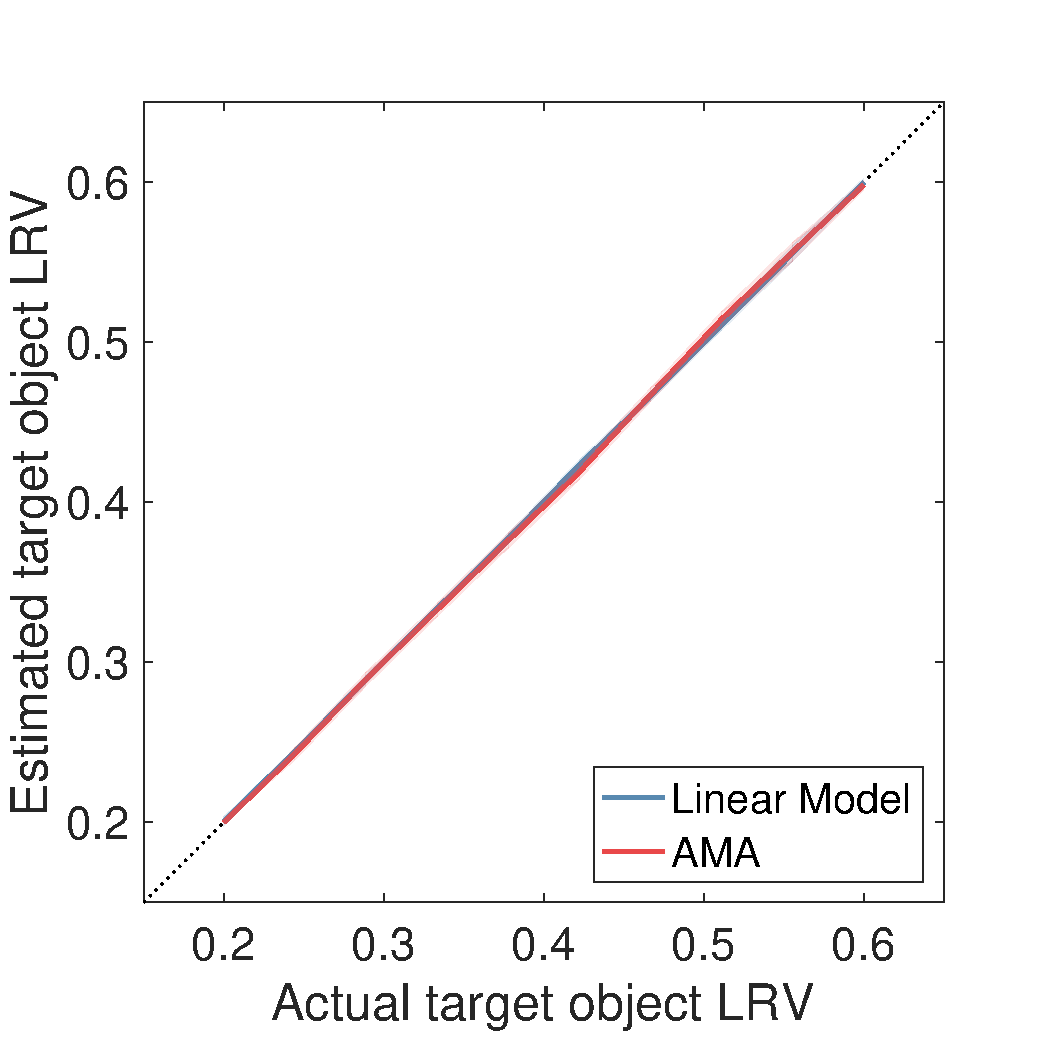
\includegraphics[width=\textwidth, trim={0 0 0 1.3cm},clip]{../FiguresDraft5/Figure10/Figure10_a.pdf}
        \label{fig:case1Estimates}
    \end{subfigure} 
        \begin{subfigure}[b]{0.26 \textwidth}
        \caption{RF responses}
        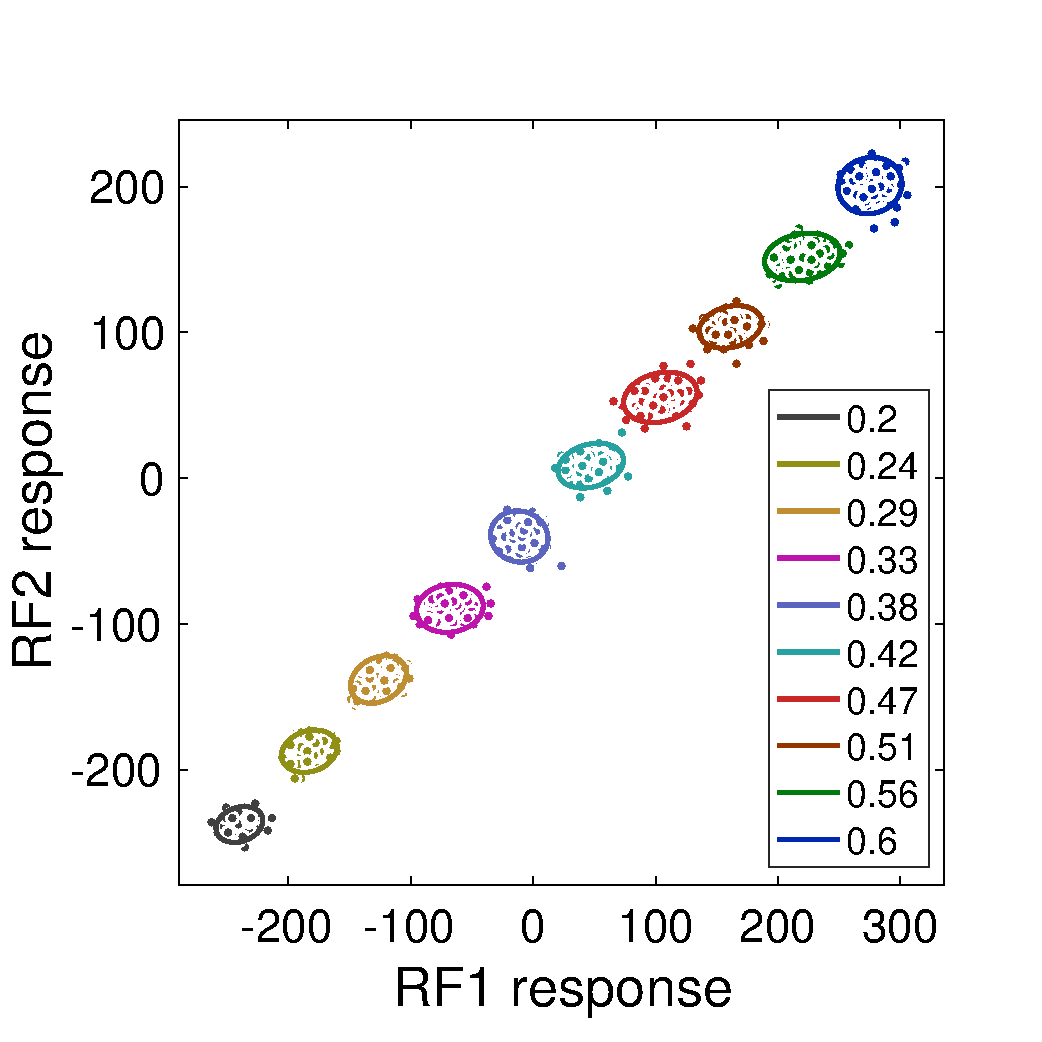
\includegraphics[width=\textwidth, trim={0 3mm 0 15mm},clip]{../FiguresDraft5/Figure10/Figure10_b.pdf}
        \label{fig:case1RFResponse}
    \end{subfigure}
    \begin{subfigure}[b]{0.4 \textwidth}
	\caption{AMA receptive fields}
	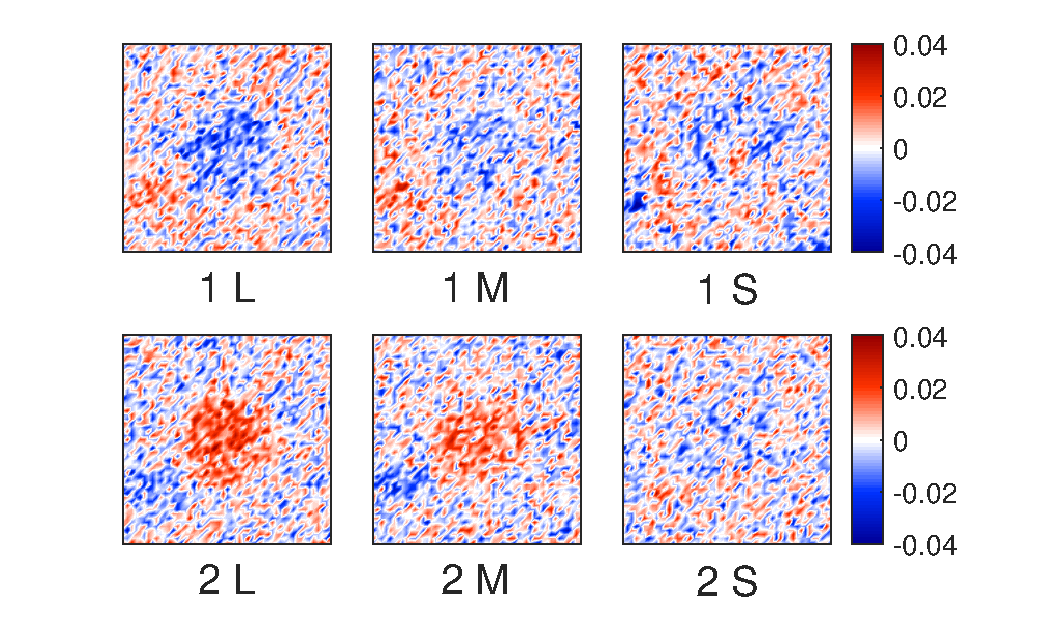
\includegraphics[width=1.0\textwidth, trim={0.2cm -0.cm 0 0.3cm}]{../FiguresDraft5/Figure10/Figure10_c.pdf}
	\label{fig:case1RFs}
    \end{subfigure}   
    \caption{{\bf Condition 1 results:} (a) Mean estimated LRV $\pm$ 1 standard deviation for images in the test set obtained using the AMA-based estimator and linear regression on the cone excitations. Solid lines show the mean estimate, the filled region in lighter color shows $\pm$ 1 standard deviation. The diagonal identity line (dotted blue) indicates veridical estimation. The standard deviations are too small to be visible. Relative RMSE (see Fig.\ref{fig:barGraphs}) is 0.7\% for linear regression and 1.1\%  for AMA based estimation. (b) Training image cone excitations in Condition 1 projected onto the first two AMA receptive fields. Each cluster of responses represents the image patches associated with a particular LRV, which is coded by color. The response clusters are approximated by a multivariate Gaussians whose mean and covariance matrices are represented by the ellipses shown in the figure. (c) The first two AMA receptive fields learned using the cone excitations of stimuli in the training set.}
\label{fig:Condition1}
\end{figure}
%% DHB, VS: In the new figure, RF1 is useless and RF2 is good.  Not the way we thought the ordering goes.  What's up?

\subsection{Condition 1}

In Condition 1, only the LRV and the relative reflectance spectrum of the target object vary across scenes.
We used accuracy maximization analysis (AMA) to learn a set of linear receptive fields that are optimal for estimating target LRV from the cone excitations to the image patches in this condition. 
Decoding performance for the test set is shown in Figure~\ref{fig:case1Estimates}. 
Figure~\ref{fig:case1Estimates} also shows the performance of the baseline linear regression method. 
Both methods are trained and tested on different image sets.
As expected, the LRV estimates obtained from decoding the AMA receptive field responses as well as the LRV estimates from linear regression are essentially perfect.

Figure~\ref{fig:case1RFResponse} shows the responses of the first two AMA receptive fields to all the image patches in the training set.
Each individual point represents the receptive field responses to an individual image patch.
Each point is color coded by the LRV corresponding to the target object in the patch.
The responses segregate nearly completely according to the target LRV, which is the feature required to support the high level 
of estimation performance shown in Figure~\ref{fig:case1Estimates}.

Figure~\ref{fig:case1RFs} shows the first two AMA receptive fields.
Each receptive field performs a weighted sum of the L, M, and S cone excitations.
The L and M cone excitations at the target object location receive large weights.
The L and M cone excitations at the background object locations and the S cone excitations at all locations receive small weights and are thus largely ignored. 
These receptive fields make sense.
For this condition, the background regions provide very little task-relevant information. 
In addition, luminance is primarily determined by L and M cones, so the S cones should make little
contribution.

The results in Figure~\ref{fig:Condition1} were obtained for one particular draw from our statistical model of illumination.
We verified that performance remained excellent for other draws.
% VS to try a few more cases to make sure.

%% DHB, VS: Maybe the above sentence is all we really need, and can delete what's below? Vijay's analysis did not actually use illuminants drawn
% from the distribution, though.
%
%% Let's just run a version Condition 1 for some other draws of illumination.
%
%For this condition, LRV estimation should be easy because the variation in target object reflectance that we introduced
%preserved LRV (which is calculated using a CIE D65 as the illumination).
%Thus, for fixed scene illuminants similar to D65, the luminance of the light reflected from the target object will vary minimally.
%In Condition 1, we used an illumination randomly sampled from our model of daylight illumination spectra (see Methods).
% and thus expect a reasonable degree of similarity to D65.
%% DHB: We need to say something about how similar.  Might explore different illuminants to dissect how sensitive the estimation
% is to whether the fixed illuminant is D65 or something else.  Probably not very, but this is an example of something we can exploit
% our graphics approach to understand, and we want to build up examples.
% JDB: I agree. The statement in current form is unnecessarily vague. With a bit of additional analysis, we could also say that different random samples produce nearly identical results, etc. etc.


%% Figure condition 2: Excitations Fail
\begin{figure}
\centering
    \begin{subfigure}[b]{0.22\textwidth}   
        \caption{\centering{LRV estimates} \newline\centering{(Excitations)}}
        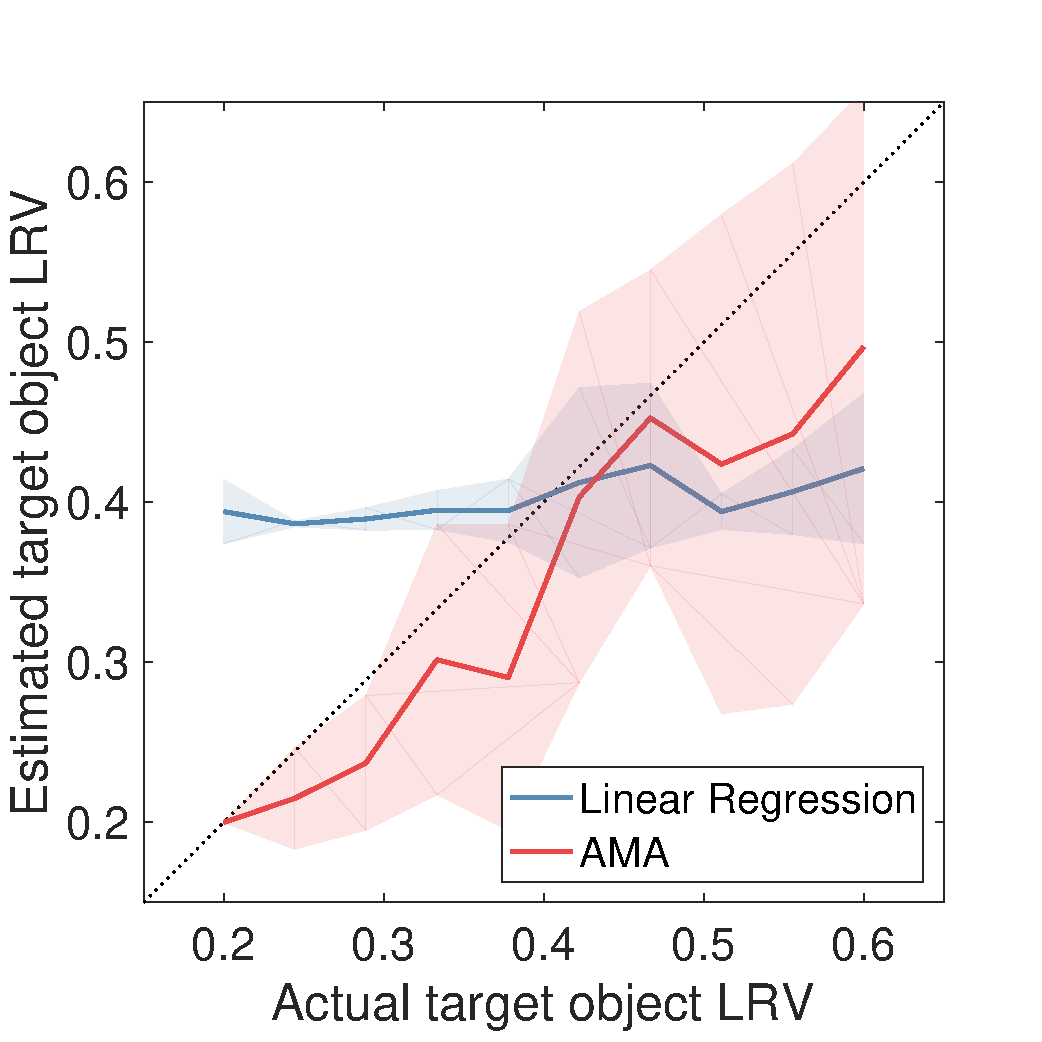
\includegraphics[width=\textwidth, trim={0 0 0 1.5cm},clip]{../FiguresDraft5/Figure11/Figure11_a.pdf}
        \label{fig:case2IsomerizationEstimates}
    \end{subfigure}
        \begin{subfigure}[b]{0.22 \textwidth}
        \caption{\centering{RF responses} \newline\centering{(Excitations)}}
        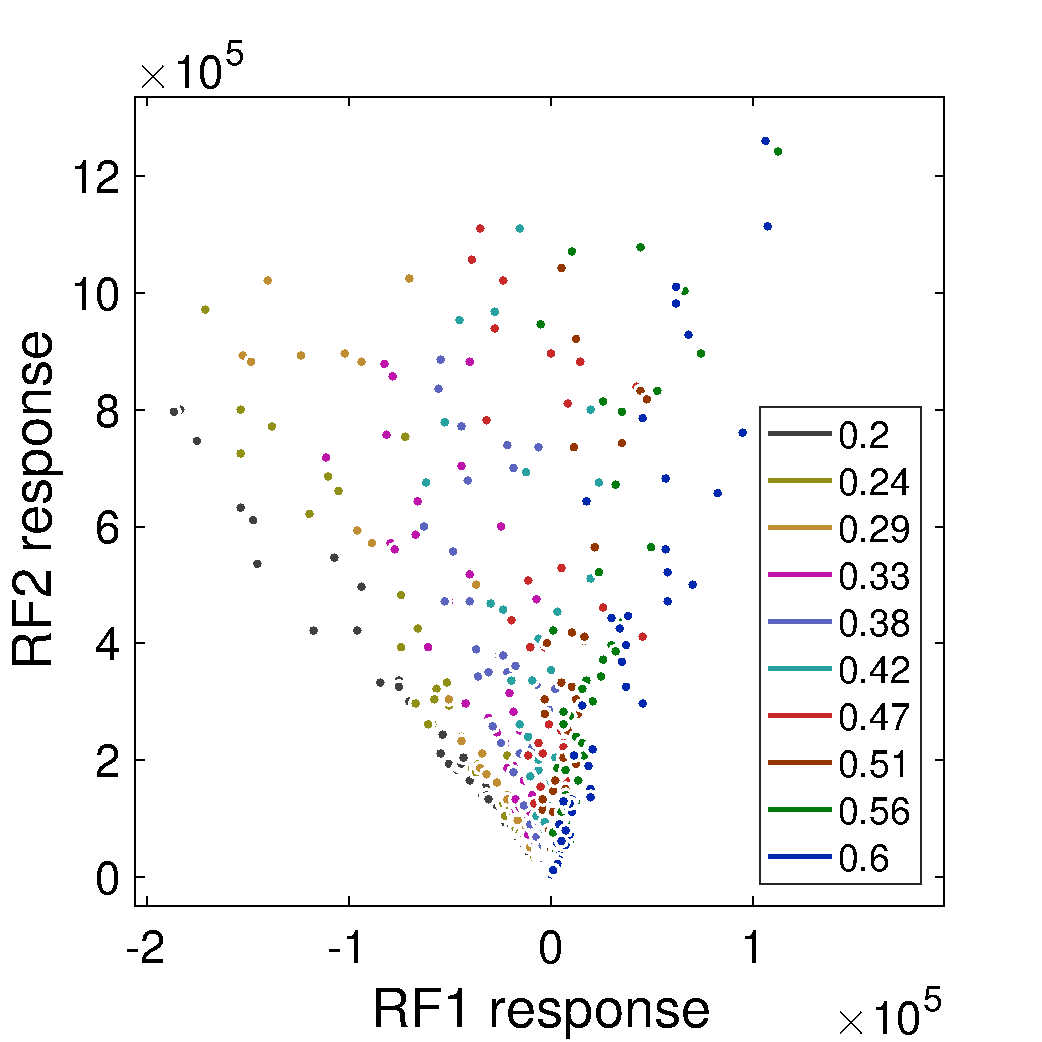
\includegraphics[width=\textwidth, trim={0 0 0 1.5cm},clip]{../FiguresDraft5/Figure11/Figure11_b.pdf}
        \label{fig:case2RFResponseIsomer}
    \end{subfigure}
            \begin{subfigure}[b]{0.22 \textwidth}
        \caption{\centering{LRV estimates}  \newline \centering{(Normalized contrast)}}
        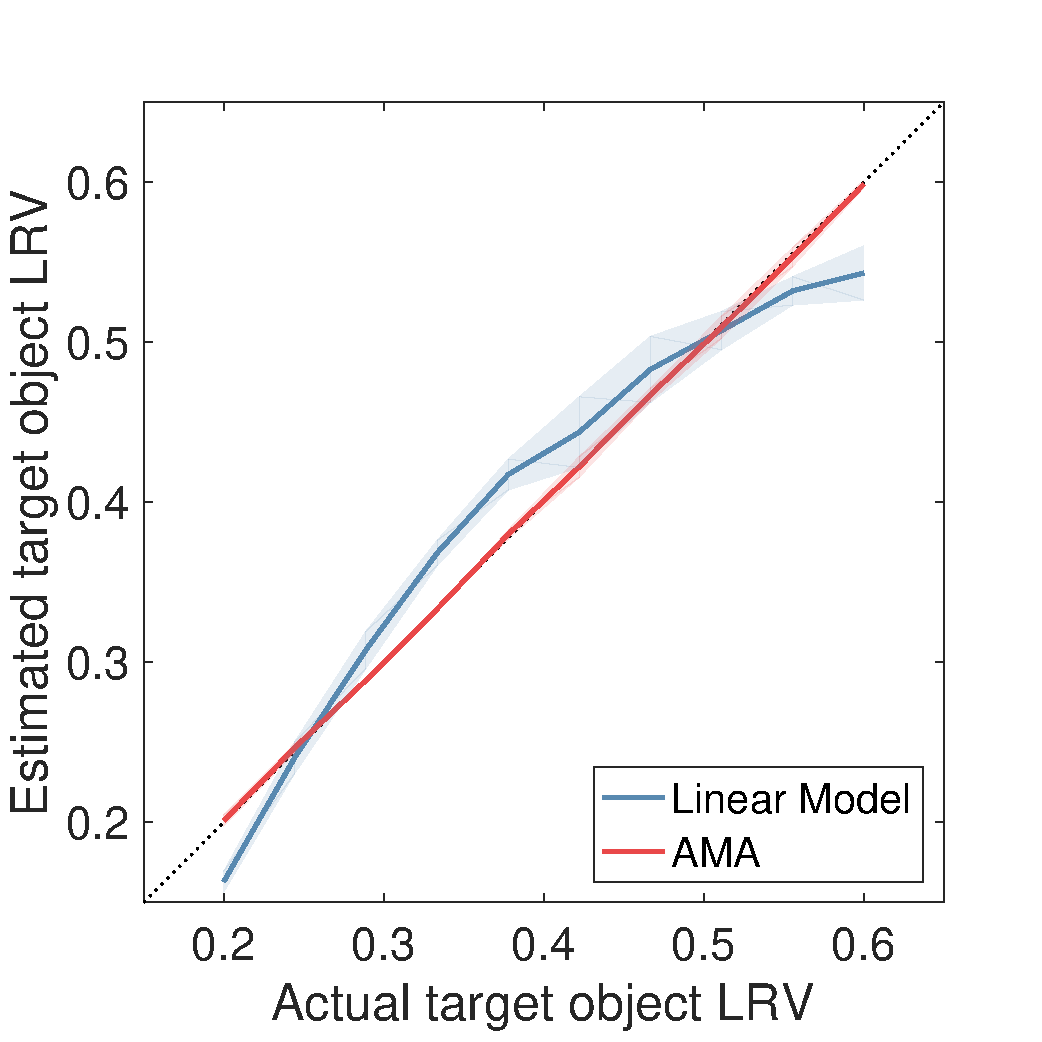
\includegraphics[width=\textwidth, trim={0 0 0 1.5cm},clip]{../FiguresDraft5/Figure11/Figure11_c.pdf}
        \label{fig:case2ContrastEstimates}
    \end{subfigure}
            \begin{subfigure}[b]{0.22 \textwidth}
        \caption{\centering{RF responses}  \newline \centering{(Normalized contrast)}}
        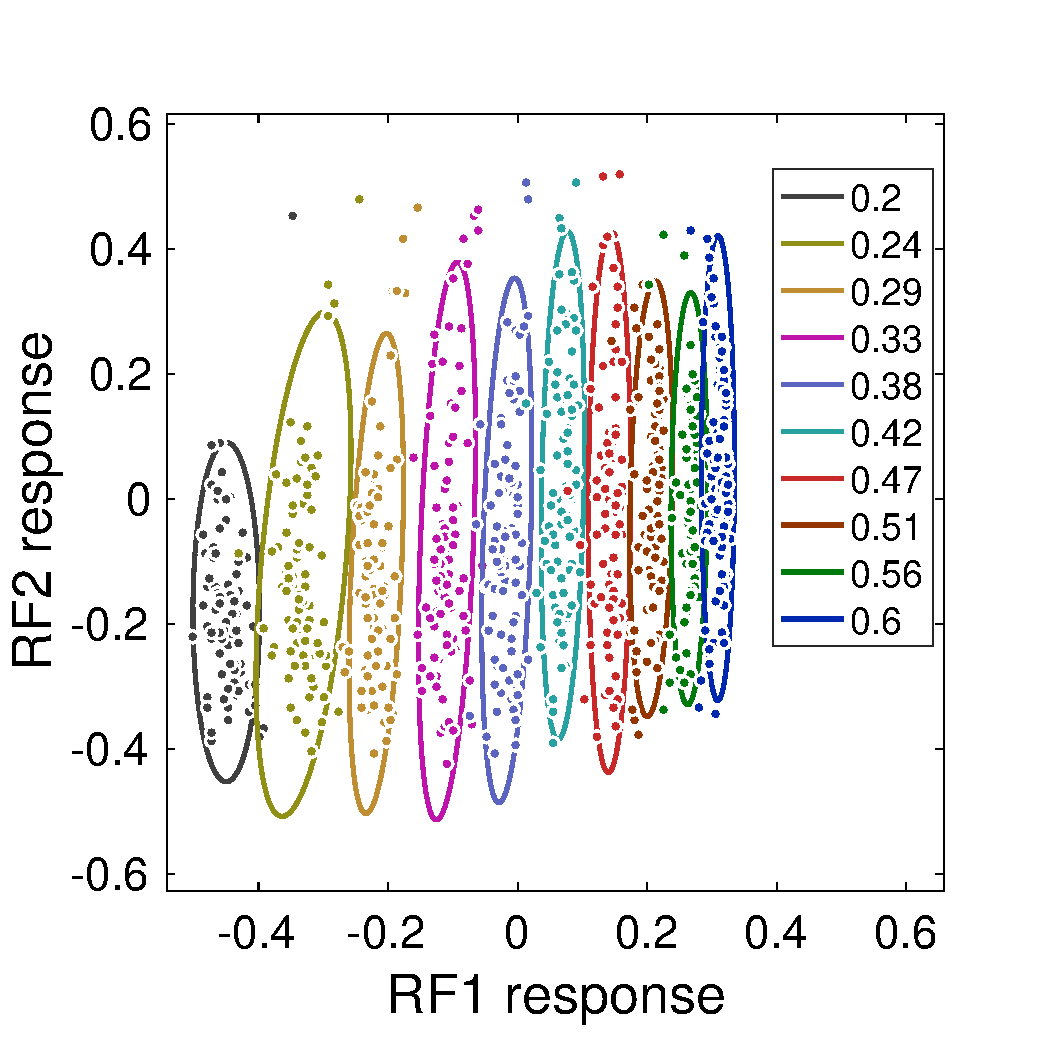
\includegraphics[width=\textwidth, trim={0 0 0 1.5cm},clip]{../FiguresDraft5/Figure11/Figure11_d.pdf}
        \label{fig:case2RFResponseContrast}
    \end{subfigure}
    \caption{{\bf Condition 2 results:} (a) Mean estimated LRV $\pm$ 1 standard deviation for images in the test set obtained using the AMA-based estimator and linear regression from the cone excitations. The relative RMSE is high (41.4\% for linear regression and 26.1\% for AMA based estimation). (b) Cone excitations projected onto AMA receptive fields. (c) Mean estimated LRV $\pm$ 1 standard deviation for images in the test set obtained using the AMA-based estimator and linear regression from the contrast normalized cone excitations. The relative RMSE of estimation is 9.3\% for linear regression and 1.6\% for AMA based estimator. (d) The contrast normalized cone excitations projected along the first two AMA receptive fields. The receptive fields were learned using AMA and the contrast normalized cone excitations. For Condition 2, the response corresponding to individual image patches at each LRV level separates much better when the input is contrast normalized cone excitations than when the input is the raw cone excitations.}
\label{fig:Condition2}
\end{figure}

\subsection{Condition 2}

Condition 2 includes variation in the spectral power distribution of the light sources, in addition to the variation present in Condition 1. 
This illumination variation makes the task more difficult because it causes additional variation in the cone excitations that is not due to target object LRV. 
We learned AMA receptive fields on the cone excitations to the images in this new condition, and again evaluated decoding performance (Fig.~\ref{fig:Condition2}(a,b)). 
Performance is poor.
Indeed, the estimates deviate considerably from the true LRV, as seen by the fact that the mean estimate
(red line) does not lie on the positive diagonal and by the fact that there is large estimation variability for each
value of the true LRV.
For this case, linear regression is also very poor. Indeed, the linear regression estimates are essentially the same as would be obtained
by simply guessing the mean LRV of the training set (0.4).

Recall that there are two qualitatively distinct factors contributing to the variation in illumination spectra: changes in overall intensity, and changes in the relative spectral power distribution. 
To separate the effect of these two factors, we trained and evaluated AMA on the contrast normalized cone excitations. 
By contrast normalizing the cone excitations, the contribution of overall intensity is essentially removed.
Figure~\ref{fig:Condition2}(c,d) shows that performance improves greatly with contrast normalization. 
Estimates obtained from the AMA receptive field responses are essentially perfect. 
Estimates obtained from linear regression are substantially improved.
This observation is consistent with previous results on computational color constancy that show that 
contrast-based representations are effective for supporting color constancy when only illumination spectra vary (e.g. \citeNP{land1986alternative}).
However, contrast-based representations are less effective at supporting constancy when the spectra of background objects in the scene vary (e.g. \citeNP{brainard1986analysis}).

%% Figure 12: Results for Condition 3
\begin{figure}
\centering
            \begin{subfigure}[b]{0.25 \textwidth}
        \caption{LRV estimates}
        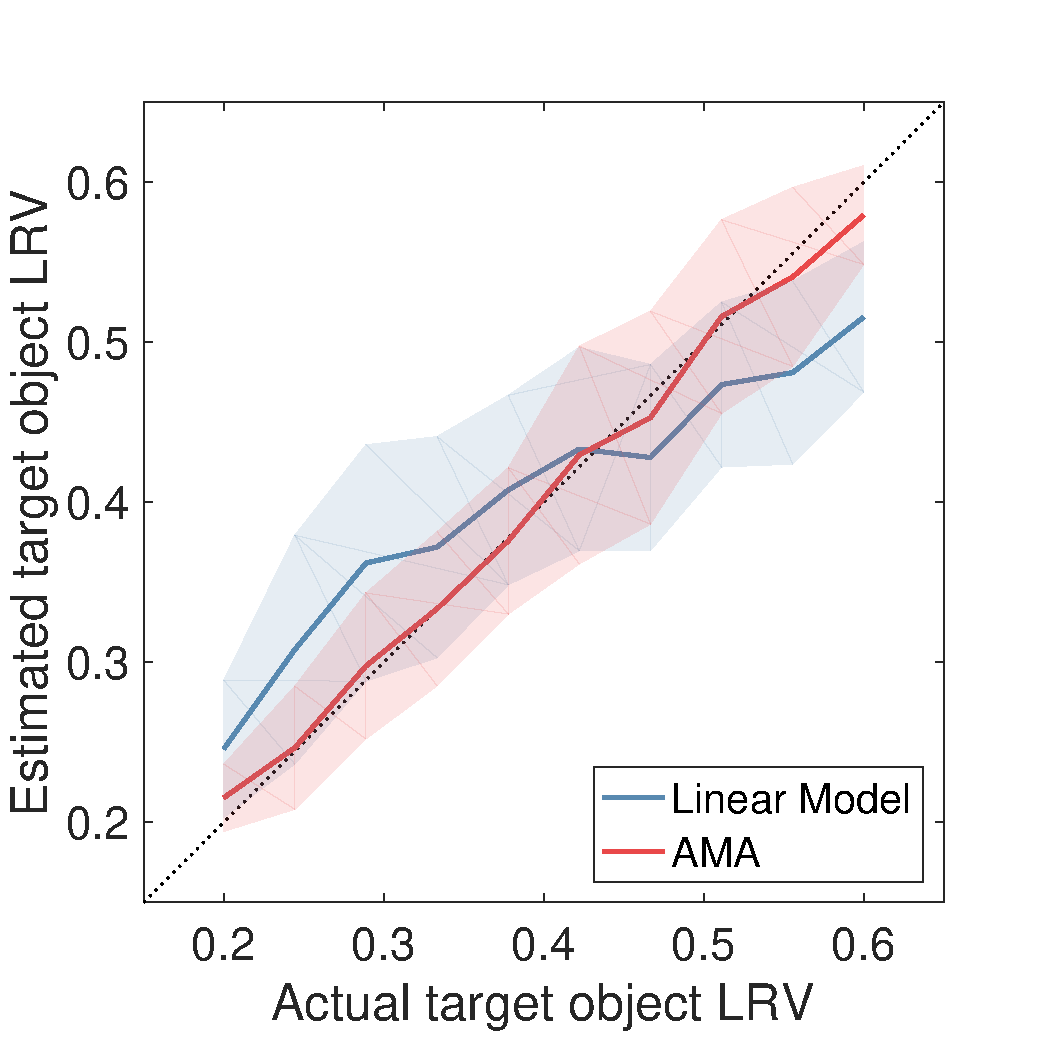
\includegraphics[width=\textwidth, trim={0 0 0 1.3cm},clip]{../FiguresDraft5/Figure12/Figure12_a.pdf}
        \label{fig:case3Estimates}
    \end{subfigure} 
        \begin{subfigure}[b]{0.26\textwidth}
        \caption{Receptive field response}
        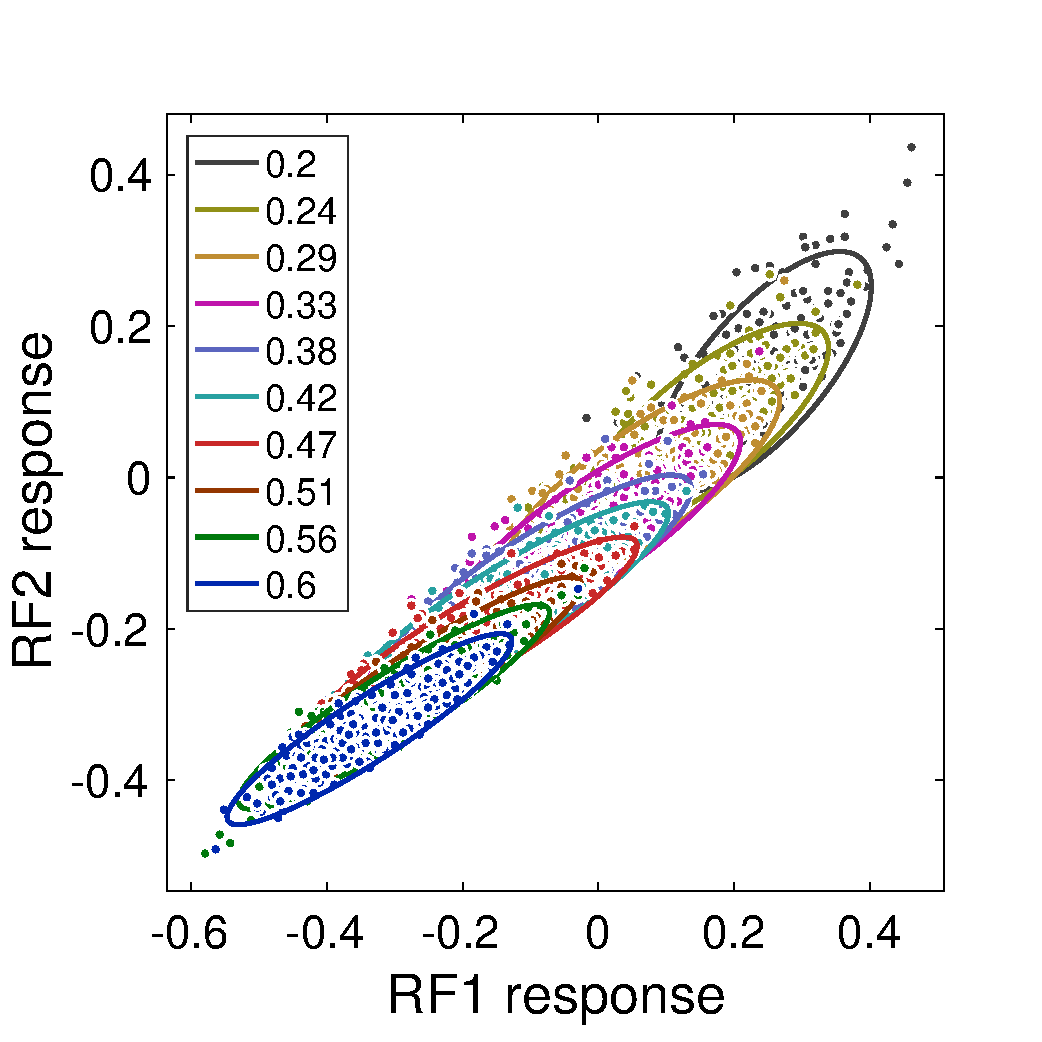
\includegraphics[width=\textwidth, trim={0 3mm 0 15mm},clip]{../FiguresDraft5/Figure12/Figure12_b.pdf}
        \label{fig:case3RFResponse}
    \end{subfigure}
    \begin{subfigure}[b]{0.4 \textwidth}
	\caption{AMA receptive fields}
	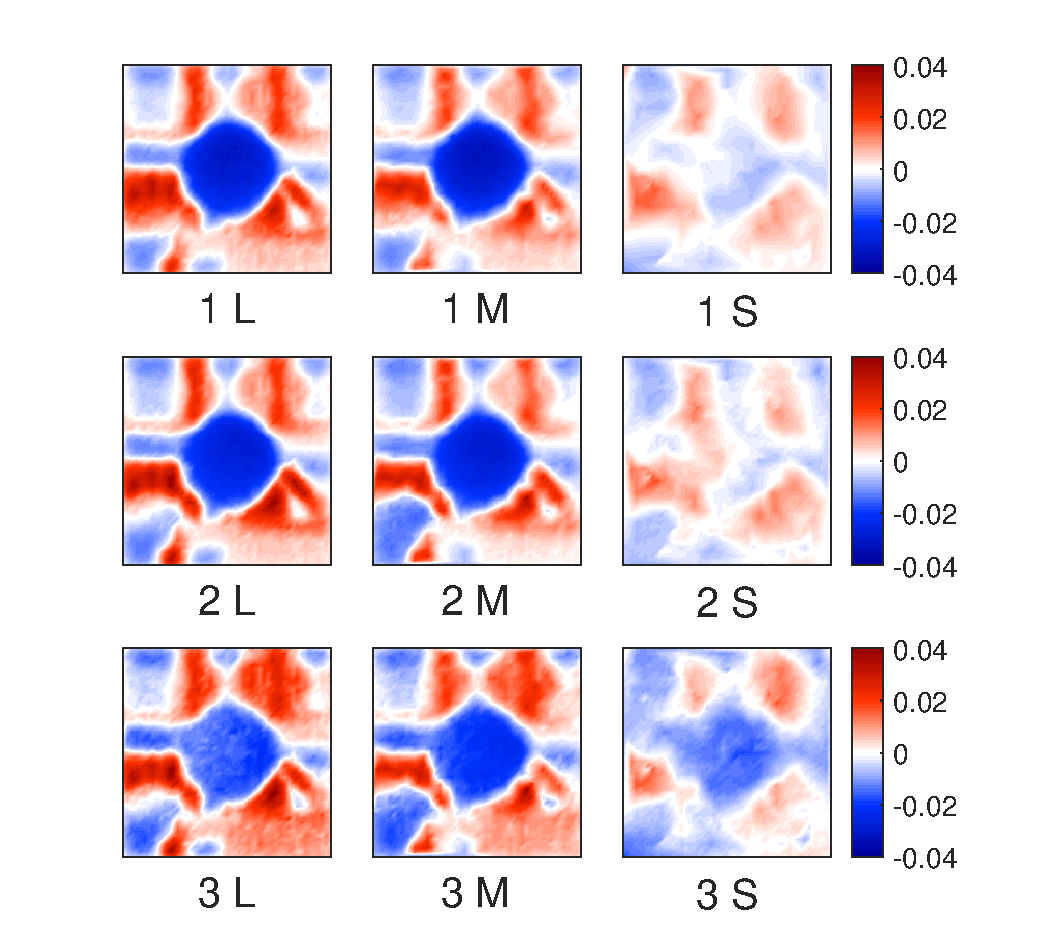
\includegraphics[width=1.0\textwidth, trim={0.2cm -0.cm 0 0.3cm}]{../FiguresDraft5/Figure12/Figure12_c.pdf}
	\label{fig:case3RFs}
    \end{subfigure}
    \caption{{\bf Condition 3 results:} (a) Mean estimated LRV $\pm$ 1 standard deviation for images in the test set obtained using the AMA-based estimator and linear regression from the contrast normalized cone excitations. The relative RMSE is 24.0\%  for linear regression and 13.1\% for AMA. (b) Contrast normalized cone excitations for the training set projected onto the first two AMA receptive fields. (c) First two AMA receptive fields learned using the contrast normalized cone excitations.}
\label{fig:Condition3}
\end{figure}

\subsection{Condition 3}

Condition 3 introduces variation in the reflectance spectra of the background objects, in addition to the sources of variation in Conditions 1 and 2.
This condition models the sources of real-world spectral variation that is most relevant for the computational problem of luminance constancy.
We again trained and evaluated AMA for labeled image patches, using the contrast normalized cone excitations.
The LRV estimates obtained via AMA are more variable and less accurate than for the previous conditions (Figure~\ref{fig:case3Estimates}).
Nevertheless, the estimates provide useful information about the target LRV.
Indeed, the estimates track the true LRV on average, as seen by the fact that the mean estimate (red line) lies along the positive diagonal.
The increased estimation variability is indicated by the increased width of the shaded red region, relative to its width for the Condition 1 and 2 results.
Performance of the baseline linear regression method (also evaluated using contrast normalized cone excitations) is worse than that of the AMA-based estimates.

Figure~\ref{fig:case3RFResponse} shows the responses of the first two AMA receptive fields to the training stimuli.
Although the responses vary systematically with target object LRV, there is considerable overlap in the receptive field responses for stimuli having different LRV values.
This overlap is due to the combined effect of the variation in the illumination and background surface spectra.
Recall, however, that the performance shown Figure~\ref{fig:case3Estimates} is based on six rather than two receptive fields;
so that there is likely to be less overlap in the full six-dimensional response space.
That is, inclusion of more receptive fields will in general reduce the ambiguity that is seen when we visualize the responses of just the first two receptive fields.
This effect is shown in the right panel of Figure~\ref{fig:RMSEvsRF}, which also illustrates the effect of training set size on estimation performance. 
%% DHB: Johannes, please check rewrite of last two sentences: OK?

% Figure RMSE vs N RFs
\begin{figure}
\centering
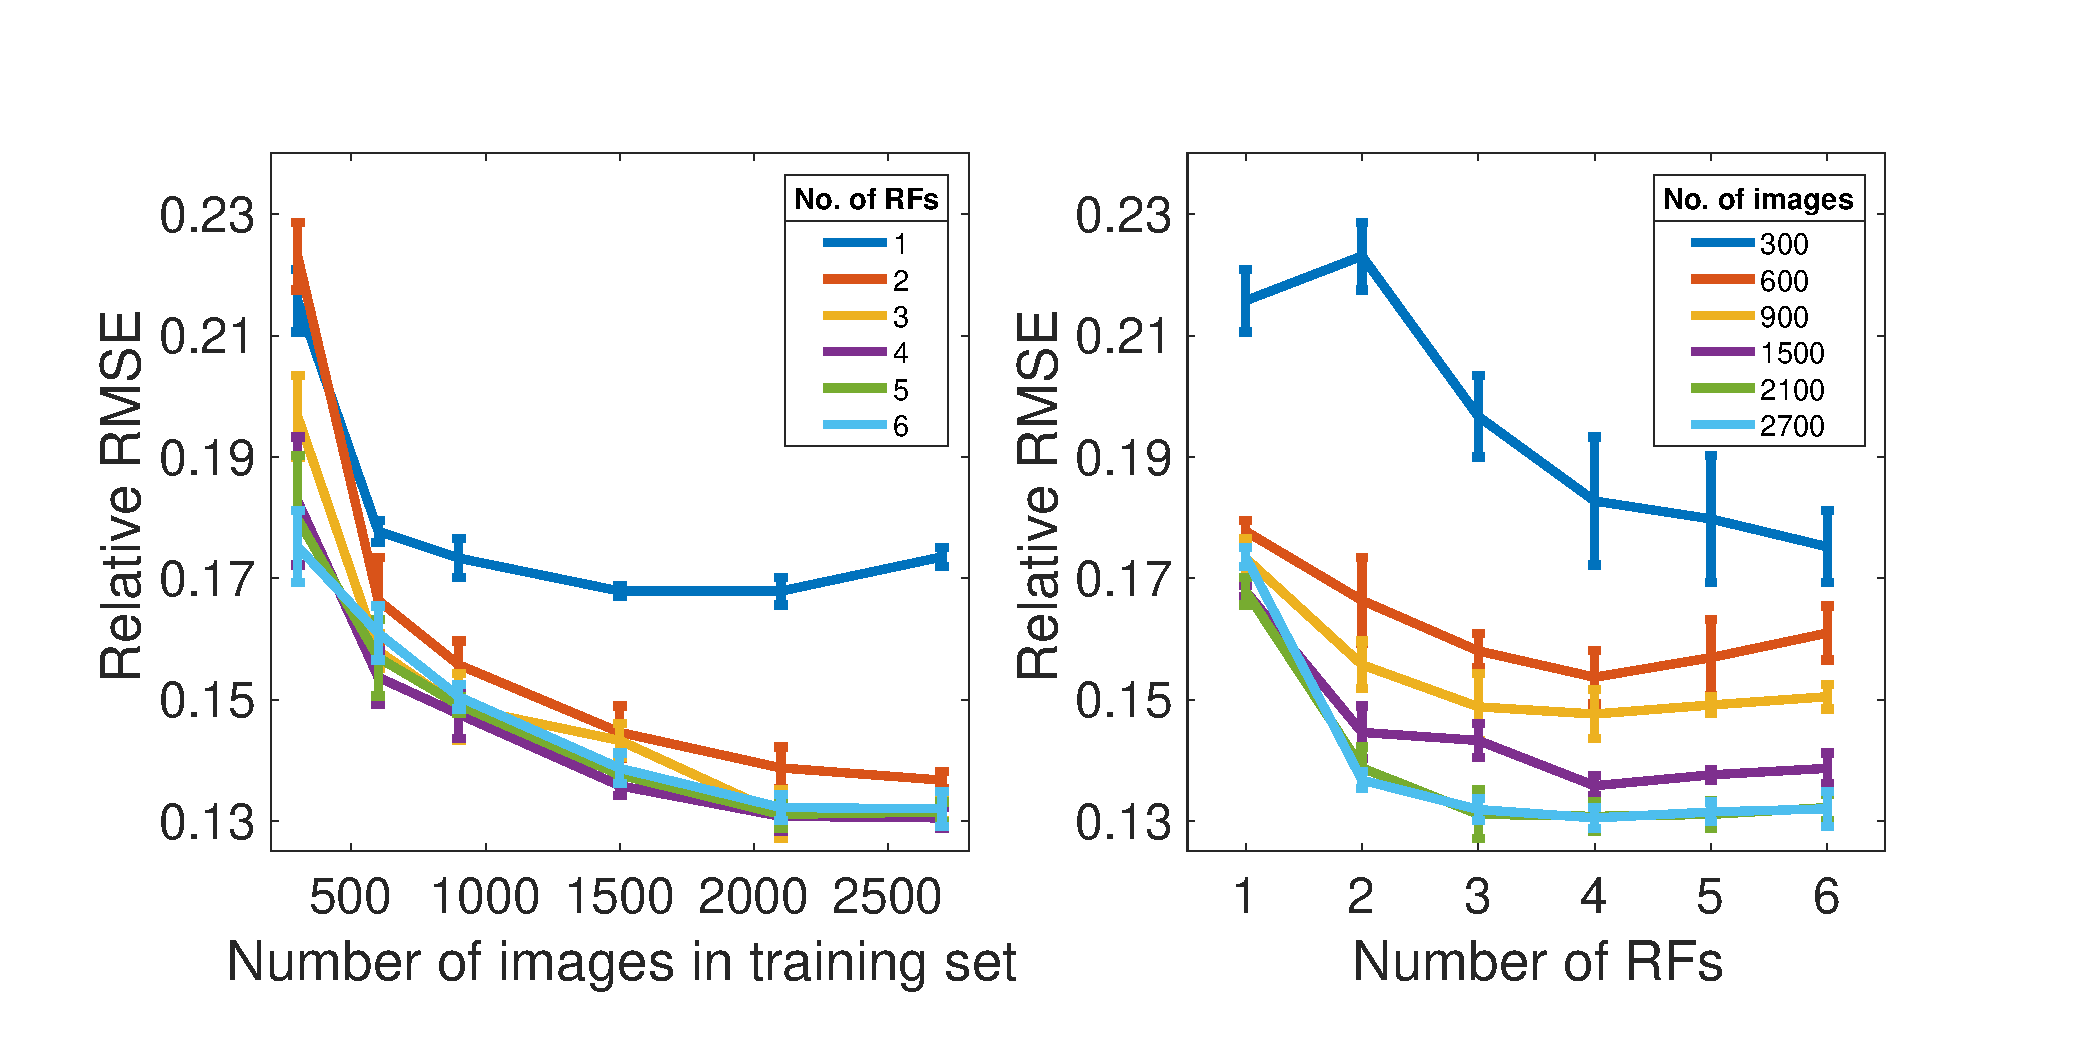
\includegraphics[width=0.6\textwidth]{../FiguresDraft5/Figure13/Figure13.pdf}
\caption{{\bf Change of relative RMSE with number of receptive fields (RFs) and size of training set:} (a) Change of relative RMSE for Condition 3 with the size of training set. The relative RMSE converges around 2000 images. To make this plot, the 300 image test set for Condition 3 was used in each case, while the training set size varied between 300 to 2700 images. The number of receptive fields used was varied between 1 and 6. (b) Same data as in a, but plotted as a function of number of receptive fields. Performance converges around 3 RFs.}
 \label{fig:RMSEvsRF}
\end{figure}

Our software allows us to compare the effect of background surface reflectances on target object LRV with and without secondary reflections from background objects. 
Our analysis shows that the secondary reflections have minimal effect on LRV estimates.
The estimates without secondary reflections are comparable to that with reflections.
This shows that the primary source of the estimation error is due to the variability in the normalized contrast of the target, due to the 
finite number of samples in the background.

Figure~\ref{fig:case3RFs} shows the first two receptive fields learned for Condition 3.
Similar to the receptive fields for Condition 1, the L and M cone excitations receive large weights, while the S cone excitations are less heavily weighted. 
Additionally, the cone excitations at the target have opposite sign compared to background object locations.
This make sense.
As discussed earlier, luminance is primarily determined by L and M cones, so the S cones should make little
contribution.
Additionally, for this condition, the optimal receptive fields compare normalized cone contrast between the target and background regions. 
This comparison may serve to reduce the effect of light scattered from the background onto the target. 
The specific geometry of the receptive fields should not be taken to be a general feature, as it arises as a consequence
of the single scene geometry we studied.
%% DHB: Let's look at RFs in case where secondary reflections are turned off, to see if what I drafted in this paragraph
% about RF structure is plausible.

\section{Discussion} \label{Discussion}

\subsection{Summary}

In this paper, we studied luminance constancy using naturalistic images.
We used a software pipeline, which was developed for this work, to render datasets of multispectral images from scene descriptions.
Because we rendered the images, we could label each image in the dataset by the light reflectance value (LRV) of the target object.
We used the labeled datasets to learn estimators for the target object LRV.
Across scenes, we varied the LRV of the target object, the relative reflectance spectrum of the target object, 
the spectral power distributions of the light sources, and the reflectance spectra of the background objects in the scene.
These spectral variations were based on statistical models of natural surface reflectance spectra and natural illumination spectra.
We studied the how the performance of the learned estimators changed with systematic manipulation of the spectral variation in the datasets.

% Figure Error Bar Graphs
\begin{figure}
\centering
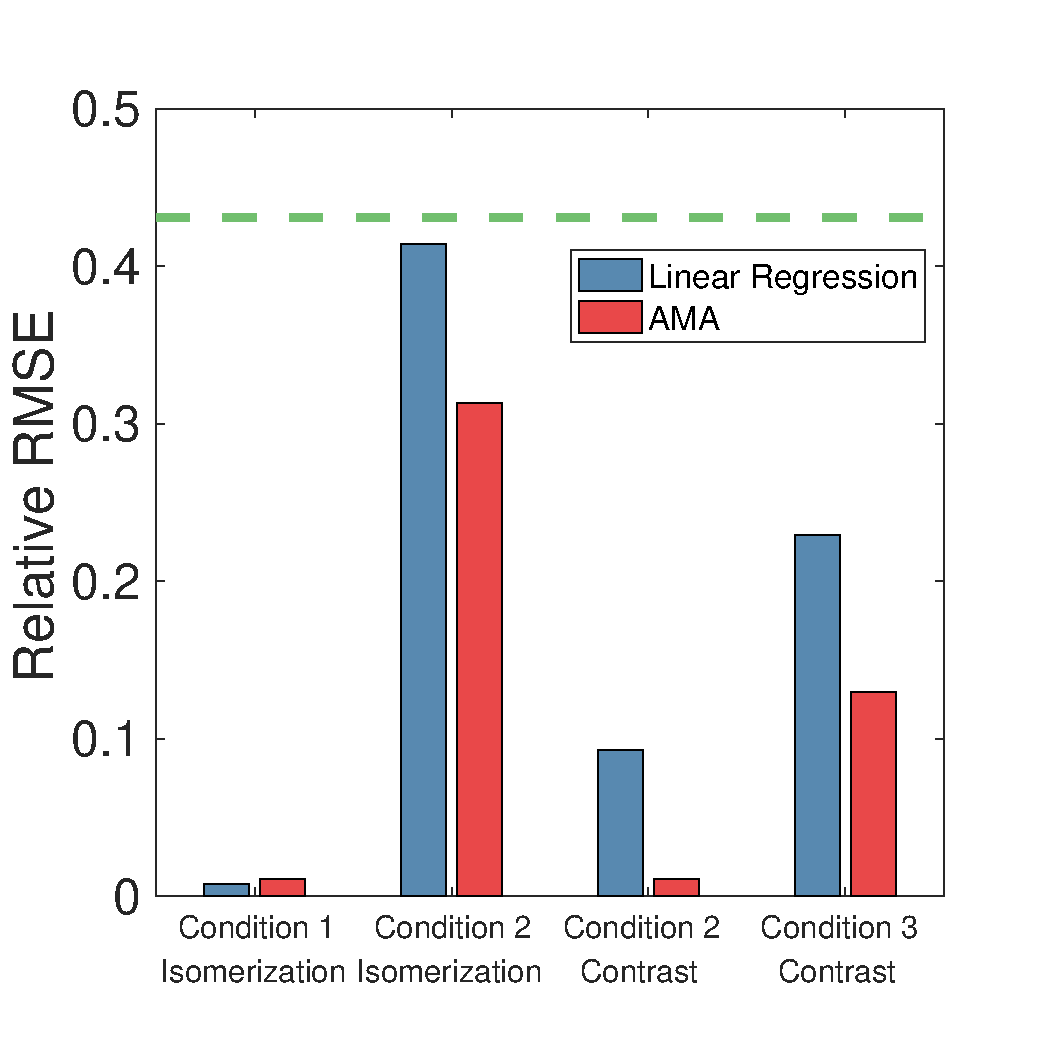
\includegraphics[width=0.3\textwidth]{../FiguresDraft5/Figure14/Figure14.pdf}
\caption{{\bf Summary of luminance constancy performance:} Relative RMSE estimation error for each method and condition. Relative RMSE is the square root of the mean of the squared difference between the estimated and true LRV divided by the true LRV. The mean is taken over all stimuli in the test set. The dotted line represents the relative RMSE for a naive method that estimates the LRV of each image as the mean LRV over the images in the set (LRV = 0.4).}
 \label{fig:barGraphs}
\end{figure}

Figure~\ref{fig:barGraphs} summarizes our main findings, by showing the overall relative root mean squared estimation error (relative RMSE; see Figure~\ref{fig:barGraphs} caption) for each condition. 
In Condition 1, where only the relative reflectance spectrum of the target object varies, 
luminance constancy is an easy computational problem,
and performance is essentially perfect for both the baseline linear regression and AMA methods.
In Condition 2, where the spectral power distribution of the illumination also varies, the problem of luminance constancy is more difficult.
Indeed, neither of our methods perform well when they operate directly on the cone excitations.
Performance with both methods improves greatly when the cone excitations are contrast normalized. 
Indeed, AMA performance for Condition 2 is essentially perfect, as it is in Condition 1.
Linear regression does less well, in part because it only has access to cone excitations at image locations
corresponding to the target object.
Condition 2, however, does not include scene-to-scene variation in the background surface reflectances,
as occurs in natural viewing.
The results for Condition 3 show performance when we add such variation.
Performance here represents the overall level of luminance constancy that our methods achieve for the
most realistic condition that we tested.
In this case, AMA-based estimates of target object LRV are, on average, within 13\% (relative RMSE) of the true value.
Introducing variation in the surface reflectance spectra of the background objects makes 
the luminance constancy problem substantially more difficult. 
Variation in the reflectance spectra of the background objects surfaces reduces how 
reliably light reflected from those objects can be used as a cue to estimate the spectral power distribution of the illuminant.
% JDB: Are we going to add in a constancy index, as we discussed doing a few meetings ago?
% DHB: I think it is time to submit this paper.

\subsection{Images of Virtual vs. Real Scenes}
As noted in the introduction, supervised learning requires large labeled datasets. Labeled datasets of natural images have been useful for developing normative models of the estimation of defocus blur, binocular disparity, retinal image motion, and 3D surface orientation \cite{burge2011optimal, burge2012optimal, burge2014optimal, burge2015optimal, kim2018lawful, burge2010natural, girshick2011cardinal, burge2016estimating, goncalves2017not}. 

Unfortunately, such datasets are not readily available for studying correlates of object surface reflectance.
To obtain ground truth information about the reflectance of objects in a natural image, it is necessary to make 
an independent measurement of the illumination impinging on each object.
Although this can be done by inserting a small number of discretely spaced reflectance standards into the scene, 
interpolating to locations between such standards requires strong assumptions.

Here we used labeled images rendered from virtual scene descriptions. 
There are many advantages to using rendered images.
One advantage is that they allow us to work with large numbers of labeled images where object reflectance is precisely known at each pixel.
A second advantage is that we can control the variation in distinct scene factors that might affect the difficulty of the estimation problem.
This flexibility allows the study of individual scene factors as well as their combined effects.
Here, we exploited this flexibility to quantify how variation in the relative reflectance spectrum of the target object, the spectrum of the illumination, and the reflectance spectrum of the background objects limit LRV estimation.
We also exploited our use of rendered images to explore how the presence or absence of secondary reflections from background objects affected estimation
of target object LRV.
This type of question cannot be addressed using real images.
The basic approach we use here can be extended to include parametric control over the amount of variation of different factors.
For example, we could systematically vary the variances of the distribution over the weights that control the relative spectrum
of the illumination.

There are also disadvantages associated with using rendered images. 
Virtual rendered scenes are not guaranteed to capture all of the task relevant variation that occurs in real scenes.
Casual inspection of our images reveals that they are rendered, and not real.
However, computer graphics is getting better and we expect that the gap between virtual and natural image databases will steadily close.
Indeed, carefully constructed graphics images are now quite difficult to differentiate from real images.

To increase the representativeness of our rendered images, we used datasets of  natural surface reflectance spectra and natural daylight illumination spectra.
Although we believe these datasets provide reasonable approximations of the statistical variation in reflectance and illumination spectra, they can be extended and improved.
For example, the surface reflectance datasets capture regularities in naturally occurring reflectance functions, but the surfaces in the datasets were not sampled to reflect the relative frequency of different reflectance spectra in natural viewing. 
In addition, the dataset of illuminations does not include the artificial illuminations that we now live much of our lives under.
Future work with virtual image datasets will benefit from targeted efforts to characterize additional features of the natural statistics of the scene components that are varied.

\subsection{Future Directions}
In the work presented here, we studied computational luminance constancy in virtual scenes with naturalistic spectral variation in light sources and in surface reflectance functions. 
It is natural to begin with spectral variation, because this variation is at the heart of what makes luminance constancy a rich computational problem.
In natural scenes, however, there are other sources of variation that add additional richness and make the problem more difficult to solve.
These include variation in non-spectral properties of objects and lighting in the scene, including object texture, material, and shape as well as lighting geometry. 
The methods we developed here may be generalized to study the effects of variation in these factors.
One could incorporate these other sources of variation into the generation of the scenes and again learn estimators from the corresponding labeled images. 
A challenge for this approach will be to thoughtfully control the increase in problem complexity, both to keep compute time feasible and to ensure that it is possible to extract meaningful insight from the results.

Luminance constancy is a special case of the more general problem of color constancy.
The approach we developed here could be generalized to the estimation of additional surface reflectance descriptors, such as object hue or chroma.
A further advance would be to develop methods for learning receptive fields that are optimal for multivariate estimation problems. 
With such methods one could directly estimate three-dimensional color descriptors.

\subsection{Linking to Human Performance}

An important motivation for studying the computational problem of luminance constancy
is to gain insight about human vision.
The approach we developed can be used to make predictions of how humans would perform in a psychophysical task that probes the visual representation of object LRV.
For example, one could study discrimination thresholds for target LRV using the stimuli that were generated with the methods used here.
More specifically, we could ask how LRV discrimination thresholds are impacted by spectral variation in the illuminant, the background objects, and in the target object itself.
Comparing human thresholds with the precision of AMA-based estimates would then allow inferences about how well human observers make use of the information available in the images for performing LRV discrimination.
We think experiments and analyses along these lines represent an important future direction.
By coupling the experiments and analyses we hope to advance, in a principled and controlled manner, our understanding of how we see objects in the real world .

\bibliography{references}
\bibliographystyle{jovcite}

\end{document}

